\documentclass[11pt]{article}

\usepackage[a4paper,margin=2.6cm]{geometry}
\usepackage[T1]{fontenc}
\usepackage{lmodern}
\usepackage{microtype}
\usepackage{amsmath,amssymb,amsthm,mathtools}
\usepackage{booktabs,array,longtable}
\usepackage{enumitem}
\usepackage{xcolor}
\usepackage{tikz}
\usetikzlibrary{arrows.meta,positioning,fit,calc}
\usepackage[colorlinks=true,linkcolor=blue!50!black,citecolor=green!35!black,urlcolor=blue!50!black]{hyperref}
\usepackage[capitalise,nameinlink]{cleveref}

\setlist{itemsep=2pt,topsep=4pt}
\allowdisplaybreaks

% ---------------------------------------------------------------- theorems
\usepackage{thmtools}
\declaretheorem[style=plain,numberwithin=section,name=Theorem]{theorem}
\declaretheorem[style=plain,sibling=theorem,name=Proposition]{proposition}
\declaretheorem[style=plain,sibling=theorem,name=Lemma]{lemma}
\declaretheorem[style=plain,sibling=theorem,name=Corollary]{corollary}
\declaretheorem[style=plain,name=Theorem,refname={Theorem,Theorems},Refname={Theorem,Theorems}]{mainthm}
\renewcommand{\themainthm}{\Alph{mainthm}}
\declaretheorem[style=definition,sibling=theorem,name=Definition]{definition}
\declaretheorem[style=definition,sibling=theorem,name=Construction]{construction}
\declaretheorem[style=remark,sibling=theorem,name=Remark]{remark}
\crefname{table}{Table}{Tables}

% ---------------------------------------------------------------- macros
\newcommand{\HOLD}{\textsf{HOLD}}
\newcommand{\RESET}{\textsf{RESET}}
\newcommand{\LOAD}{\textsf{LOAD}}
\newcommand{\FAV}[1]{\textsf{FAVOR}(#1)}
\newcommand{\NORMAL}{\textsf{NORMAL}}
\newcommand{\MAJ}{\operatorname{MAJ}}
\newcommand{\AND}{\operatorname{AND}}
\newcommand{\OR}{\operatorname{OR}}
\newcommand{\Pred}{\textsc{Pred}_4\textsc{-Tree}}
\newcommand{\Ever}{\textsc{Ever}_4\textsc{-Tree}}
\newcommand{\EVAL}{\textsc{Mslp-Eval}}
\newcommand{\OMCVP}{\textsc{Omcvp}}
\newcommand{\one}{\mathbf{1}}
\newcommand{\kend}{\kappa_{\mathrm{end}}}
\newcommand{\val}{\operatorname{val}}
\newcommand{\dist}{\operatorname{dist}}
\newcommand{\rank}{\operatorname{rank}}
\newcommand{\ep}[2]{#1^{#2}}          % endpoint of cell #1 adjacent to #2
\newcommand{\Lsp}{\mathsf{L}}
\newcommand{\Ptime}{\mathsf{P}}
\newcommand{\NC}{\mathsf{NC}}
\newcommand{\prim}[1]{\textsf{#1}}
\newcommand{\Hz}{H}
\newcommand{\Word}{w}
\newcommand{\ie}{i.e.}

\title{P-Completeness of Synchronous Majority on Trees of Maximum Degree Four:\\
a Modular Proof via Monotone Boolean Straight-Line Programs}
\author{}
\date{Consolidated version, 13 November 2026}

\begin{document}
\maketitle

\begin{abstract}
We consider synchronous majority dynamics on an explicitly given finite tree: every vertex
simultaneously adopts the strict majority of its neighbours' bits and keeps its own bit on a tie.
We prove that predicting the state of a designated vertex at a binary-encoded time is
$\Ptime$-complete under logspace many-one reductions, already on trees of maximum degree four whose
vertex degrees all lie in $\{1,3,4\}$. Deciding whether a designated, initially zero vertex ever
becomes one is $\Ptime$-complete as well.

The proof is organised around a single \emph{simulation theorem}: a logspace transducer turns every
monotone Boolean straight-line program into a tree of maximum degree four, an initial configuration,
a designated vertex and an observation time, such that the majority evolution reproduces the value
of the program's designated register. The physical tree is a serial processor whose memory cells,
transport junctions, logic gates and non-destructive reader are all driven by private autonomous
control trees; no state is forced from outside during the evolution. The simulation is assembled
from local contracts, a phase calculus that certifies every control word, and explicit invariants
composed by induction over the program. For a program with $m$ registers the observation time is
$O(m^2)$ and the tree has $O(m^{13})$ vertices.

This is a consolidated, reorganised presentation of an existing proof. All substantive mathematical
content of the original manuscript is retained; \cref{app:map} maps each result to its source.
\end{abstract}

\setcounter{tocdepth}{2}
\tableofcontents

% ====================================================================
\section{Introduction}\label{sec:intro}
% ====================================================================

\subsection{The problem and the results}

Let $T=(V,E)$ be a finite simple undirected tree in which every vertex carries a bit. In
\emph{synchronous majority dynamics} all vertices update at the same time: a vertex takes the strict
majority of the bits of its neighbours, and keeps its own bit when the neighbours are tied. There are
no weights, no directed edges and no physical self-loops. We study two decision problems for this
dynamics on trees of maximum degree four (formal definitions are in \cref{sec:prelim}):
\begin{itemize}
\item $\Pred$: given the tree, an initial configuration, a vertex $v^\ast$ and a time $\tau$ written
  in binary, is $v^\ast$ in state $1$ at time $\tau$?
\item $\Ever$: given the tree, an initial configuration and a vertex $z$ initially in state $0$, is
  $z$ in state $1$ at some time?
\end{itemize}

The heart of the paper is the following simulation theorem, stated precisely as
\cref{thm:simulation}. Monotone Boolean straight-line programs are defined in \cref{sec:model}.

\begin{mainthm}[Simulation theorem]\label{thmA}
There is a logspace transducer that maps every monotone Boolean straight-line program $\mathcal P$
to a tree $T$ of maximum degree four, an initial configuration, a vertex $v^\ast$ and a time $\tau$
written in binary, such that the state of $v^\ast$ at time $\tau$ under synchronous majority equals
the final value of the designated register of $\mathcal P$. If $\mathcal P$ has $m$ registers in
single-assignment normal form, then $\tau=O(m^2)$, $|V(T)|=O(m^{13})$, and all vertex degrees lie in
$\{1,3,4\}$. A variant of the construction produces, instead of $(v^\ast,\tau)$, a vertex $z$
initially in state $0$ which is ever in state $1$ if and only if the program outputs $1$.
\end{mainthm}

Combined with the classical $\Ptime$-completeness of monotone circuit value (\cref{sec:pcomplete})
and with the classical bounded-transient behaviour of symmetric majority networks
(\cref{sec:membership}), the simulation theorem gives the two completeness results.

\begin{mainthm}\label{thmB}
$\Pred$ is $\Ptime$-complete under logspace many-one reductions. Hardness already holds for trees
whose vertex degrees all belong to $\{1,3,4\}$, with a query time polynomial in the instance size.
\end{mainthm}

\begin{mainthm}\label{thmC}
$\Ever$ is $\Ptime$-complete under logspace many-one reductions, already on trees whose vertex
degrees all belong to $\{1,3,4\}$.
\end{mainthm}

Since trees have treewidth one, hardness holds at treewidth one. The results say nothing about
maximum degree three; see \cref{rem:scope}.

\subsection{Architecture of the proof}\label{sec:architecture}

The proof has six parts, each in its own section.
\begin{enumerate}[label=(\arabic*)]
\item \emph{Computational model} (\cref{sec:model}). Monotone Boolean straight-line programs:
  Boolean registers, $\AND$/$\OR$ instructions, unrestricted reuse of stored values, and no
  conditional jumps. A logspace normal form gives single assignment and topological order.
\item \emph{$\Ptime$-completeness of program evaluation} (\cref{sec:pcomplete}). This is
  essentially the classical result of Ladner and Goldschlager. We do not reprove it.
\item \emph{Simulation theorem} (\cref{sec:simulation}). We state it and split its proof into
  two layers. The first is a \emph{controlled processor}, whose control vertices follow prescribed
  words. The second consists of \emph{autonomous clocks} that generate those words. A substitution
  principle (\cref{prop:substitution}) glues the layers.
\item \emph{Modular simulation lemmas}:
  \begin{itemize}
  \item storage, transport, logic and reading, as local contracts (\cref{sec:modules});
  \item clocks and synchronisation, through a phase calculus and robust generators
    (\cref{sec:clocks});
  \item restoration and composition, through explicit invariants and induction over the program
    (\cref{sec:processor}).
  \end{itemize}
\item \emph{Reduction analysis} (\cref{sec:analysis}): correctness, size, time, degree, acyclicity
  and logspace constructibility.
\item \emph{Completeness results} (\cref{sec:completeness}). Membership in $\Ptime$ is proved
  separately, and eventual activation is treated as an additional result with its own
  finite-window reader.
\end{enumerate}

\Cref{fig:dependencies} shows how the results depend on each other. An arrow $X\to Y$ means that the
proof of $Y$ uses $X$.

\begin{figure}[ht]
\centering
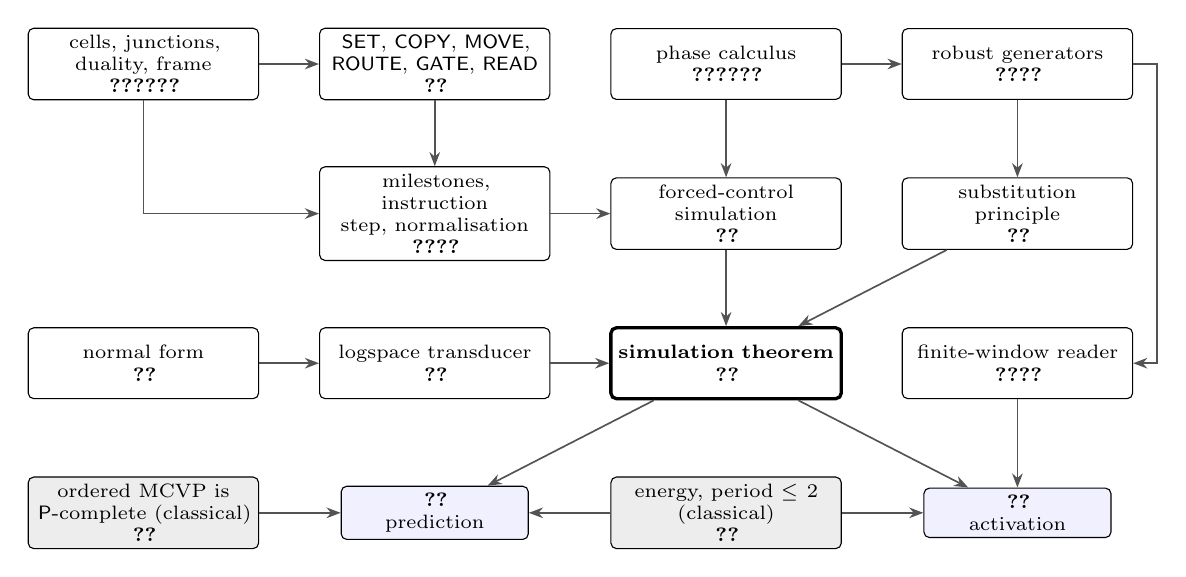
\begin{tikzpicture}[
  box/.style={draw,rounded corners=2pt,align=center,font=\scriptsize,inner sep=2.5pt,
              text width=2.75cm,minimum height=9mm},
  cls/.style={box,fill=gray!14},
  main/.style={box,fill=blue!6,text width=2.2cm,minimum height=6mm},
  arr/.style={-{Stealth[length=1.8mm]},semithick,gray!65!black}]
\def\xa{0}\def\xb{3.7}\def\xc{7.4}\def\xd{11.1}
% row 1: local modules and clocks
\node[box] (cell)  at (\xa,0) {cells, junctions,\\ duality, frame\\ \cref{lem:modes,lem:duality,lem:frame}};
\node[box] (prims) at (\xb,0) {\prim{SET}, \prim{COPY}, \prim{MOVE},\\ \prim{ROUTE}, \prim{GATE}, \prim{READ}\\ \cref{sec:modules}};
\node[box] (phase) at (\xc,0) {phase calculus\\ \cref{lem:cellphase,lem:concat,lem:timing}};
\node[box] (gens)  at (\xd,0) {robust generators\\ \cref{thm:phasedefect,cor:words}};
% row 2: composition
\node[box] (proc)  at (\xb,-1.9) {milestones, instruction\\ step, normalisation\\ \cref{prop:instruction,lem:normalize}};
\node[box] (forced) at (\xc,-1.9) {forced-control\\ simulation\\ \cref{thm:forced}};
\node[box] (subst) at (\xd,-1.9) {substitution\\ principle\\ \cref{prop:substitution}};
% row 3: the simulation theorem
\node[box] (nf)    at (\xa,-3.8) {normal form\\ \cref{lem:normalform}};
\node[box] (logsp) at (\xb,-3.8) {logspace transducer\\ \cref{prop:logspace}};
\node[box,very thick] (sim) at (\xc,-3.8) {\textbf{simulation theorem}\\ \cref{thm:simulation}};
\node[box] (reader) at (\xd,-3.8) {finite-window reader\\ \cref{lem:reader,lem:finalwrite}};
% row 4: classical inputs and main results
\node[cls] (mcvp)   at (\xa,-5.7) {ordered MCVP is\\ $\Ptime$-complete (classical)\\ \cref{thm:mcvp}};
\node[main] (B)     at (\xb,-5.7) {\textbf{\cref{thmB}}\\ prediction};
\node[cls] (energy) at (\xc,-5.7) {energy, period $\le2$\\ (classical)\\ \cref{prop:membership}};
\node[main] (C)     at (\xd,-5.7) {\textbf{\cref{thmC}}\\ activation};
% arrows
\draw[arr] (cell) -- (prims);
\draw[arr] (prims) -- (proc);
\draw[arr] (cell.south) |- (proc.west);
\draw[arr] (phase) -- (gens);
\draw[arr] (phase) -- (forced);
\draw[arr] (proc) -- (forced);
\draw[arr] (gens) -- (subst);
\draw[arr] (forced) -- (sim);
\draw[arr] (subst) -- (sim);
\draw[arr] (nf) -- (logsp);
\draw[arr] (logsp) -- (sim);
\draw[arr] (gens.east) -- ++(0.3,0) |- (reader.east);
\draw[arr] (sim) -- (B);
\draw[arr] (sim) -- (C);
\draw[arr] (reader) -- (C);
\draw[arr] (mcvp) -- (B);
\draw[arr] (energy) -- (B);
\draw[arr] (energy) -- (C);
\end{tikzpicture}
\caption{Dependencies between the main results. Shaded boxes are classical results that we cite.}
\label{fig:dependencies}
\end{figure}

\subsection{Classical results and original contributions}\label{sec:credits}

We cite the following results and do not reprove them, except where a short proof is needed in the
exact form we use.
\begin{itemize}
\item $\Ptime$-completeness of the circuit value problem for circuits presented as straight-line
  sequences \cite{Lad75}, and of its monotone restriction \cite{Gol77}; see also
  \cite[Appendix~A.1]{GHR95}. This is \cref{thm:mcvp}.
\item Closure of logspace reductions under composition \cite{Jon75,LL76}.
\item Period at most two and a linear transient for symmetric threshold networks, proved with a
  bounded energy function \cite{GO80,PS83,GFP85}. We include the short proof in
  \cref{prop:membership}, because we need the explicit transient bound for binary-encoded times.
\end{itemize}

The following constructions and results come from the original manuscript~\cite{Src}. To our
knowledge they are not in the classical literature:
\begin{itemize}
\item robust tree generators of all phase-defect words, with degree at most four and polynomial
  size, constructible in logspace (\cref{sec:generators});
\item the two-vertex \textsf{EDGE} memory cell with modes \RESET/\HOLD/\LOAD, and the local
  operations \prim{MOVE}, \prim{ROUTE} and the five-transition gates (\cref{sec:modules});
\item the fourteen-transition non-destructive reader that restores its isolating cells
  (\cref{lem:read});
\item the serial tree processor, its normal configurations, and the background normalisation wave
  (\cref{sec:processor});
\item the finite-window reader and the special final write used for eventual activation
  (\cref{sec:ever}).
\end{itemize}

This version reorganises the proof and adds the following organisational lemmas, each proved here:
\begin{itemize}
\item a mode-level duality lemma (\cref{lem:duality});
\item a frame lemma (\cref{lem:frame});
\item a cell-phase lemma (\cref{lem:cellphase});
\item a concatenation lemma that excludes the merging of control blocks (\cref{lem:concat});
\item a table of timing signatures of all primitives (\cref{tab:timing});
\item the substitution principle (\cref{prop:substitution});
\item an explicit list of milestone configurations (\cref{tab:milestones});
\item a closed formula for the observation time (\cref{prop:instruction,cor:tau}).
\end{itemize}
\Cref{app:map} records the correspondence with the original manuscript, and \cref{app:audit} lists
the points that the reorganisation made explicit.

\subsection{Conventions}\label{sec:conventions}

We write $\oplus$ for exclusive or. For an integer $t$, its \emph{parity} is $t\bmod 2$. For a
statement $S$, $\one\{S\}\in\{0,1\}$ is its indicator. For integers $a\le b$, $[a,b)$ is the set of
integers $t$ with $a\le t<b$.

A configuration at \emph{state time} $t$ is the vector of all bits at time $t$. A bit that a
vertex reads at state time $t$ is called a \emph{control value at control time $t$}: it influences
the transition from state time $t$ to state time $t+1$. In schedules, \emph{``during $[s,s+\ell)$''}
refers to control times. An operation occupying the control times $[s,s+\ell)$ takes the
configuration at state time $s$ to the configuration at state time $s+\ell$, and has
\emph{duration} $\ell$.

% ====================================================================
\section{Preliminaries on majority dynamics}\label{sec:prelim}
% ====================================================================

\begin{definition}[Synchronous majority]\label{def:majority}
Let $T=(V,E)$ be a finite simple undirected graph and $x(0)\in\{0,1\}^V$. For $t\ge 0$ and $v\in V$
with neighbourhood $N(v)$, put $n_1=|\{u\in N(v):x_u(t)=1\}|$ and $n_0=|N(v)|-n_1$, and define
\[
x_v(t+1)=\begin{cases}1&\text{if } n_1>n_0,\\ 0&\text{if } n_1<n_0,\\ x_v(t)&\text{if } n_1=n_0.\end{cases}
\]
\end{definition}

For $k$ odd, $\MAJ_k$ denotes the majority of $k$ bits. In this paper only degrees one to four occur.
A vertex of degree one copies its neighbour, and a vertex of degree three takes $\MAJ_3$ of its
neighbours, with no self-vote at odd degree. At degree four the rule is equivalent to
\begin{equation}\label{eq:maj5}
x_v(t+1)=\MAJ_5\bigl(x_v(t),x_{u_1}(t),x_{u_2}(t),x_{u_3}(t),x_{u_4}(t)\bigr),
\end{equation}
because a tie $2$--$2$ among the neighbours is broken by $x_v(t)$, and a $3$--$1$ or $4$--$0$ split
is not affected by one extra vote. The old state is used \emph{only} to implement the tie rule. It is
not an additional programmable neighbour. In particular, it is never a ``fifth physical
neighbour''.

\begin{lemma}[Self-duality]\label{lem:selfdual}
If $x(\cdot)$ is a trajectory of synchronous majority on $T$, then so is its complement
$\bar x(t)=\mathbf 1-x(t)$.
\end{lemma}

\begin{proof}
Complementing all neighbours swaps $n_0$ and $n_1$. The tie rule is complemented together with the
old state.
\end{proof}

We often analyse a set $U\subseteq V$ while treating the vertices outside $U$ as given signals.

\begin{definition}[Open evolution]\label{def:open}
Let $U\subseteq V$, and let $\partial U$ be the set of vertices outside $U$ that are adjacent to
some vertex of $U$. Given initial bits on $U$ and a \emph{boundary history} $y:\partial U\times\mathbb N\to\{0,1\}$,
the \emph{open evolution} of $U$ applies \cref{def:majority} to every $v\in U$, using $y_u(t)$ as the
state of $u\in\partial U$ at time $t$.
\end{definition}

\begin{lemma}[Locality]\label{lem:locality}
Let $x(\cdot)$ be a trajectory of the whole graph. For every $U\subseteq V$, the restriction of $x$
to $U$ coincides with the open evolution of $U$ from $x(0)|_U$ under the boundary history
$y_u(t)=x_u(t)$. Consequently, two trajectories that agree on $U$ at time $0$ and on $\partial U$ at
all times $0\le t<t_1$ agree on $U$ at all times $0\le t\le t_1$.
\end{lemma}

\begin{proof}
Both claims follow by induction on $t$, because the update of $v\in U$ at time $t$ reads only
$x_v(t)$ and the states at time $t$ of the neighbours of $v$, which lie in $U\cup\partial U$.
\end{proof}

\Cref{lem:locality} is used constantly, often implicitly. In the following sections a typical
statement is: ``for every history of the port $u$, the vertices of $U$ do the following''. Such a
statement is a claim about the open evolution of $U$ for \emph{every} boundary history. By
\cref{lem:locality} it applies to the actual history, whatever that turns out to be, including
histories that depend on the past states of $U$ through feedback.

\begin{definition}[Decision problems]\label{def:problems}
An instance of $\Pred$ consists of an explicit tree $T$ of maximum degree at most four, listed by
its vertices and edges, an initial configuration $x(0)$, a vertex $v^\ast$, and a nonnegative
integer $\tau$ encoded in binary. The question is whether $x_{v^\ast}(\tau)=1$.

An instance of $\Ever$ consists of such a tree and configuration, together with a vertex $z$ with
$x_z(0)=0$. The question is whether $x_z(t)=1$ for some $t\ge 1$.
\end{definition}

% ====================================================================
\section{The computational model: monotone Boolean straight-line programs}\label{sec:model}
% ====================================================================

\begin{definition}[Monotone Boolean straight-line program]\label{def:mslp}
A \emph{monotone Boolean straight-line program} (MSLP) is a tuple
$\mathcal P=(r,\iota_0,(\pi_1,\dots,\pi_L),o)$ where:
\begin{itemize}
\item $r\ge 1$ is the number of \emph{registers} $R_1,\dots,R_r$, each holding one bit;
\item $\iota_0\in\{0,1\}^r$ is the \emph{initial content} of the registers;
\item each \emph{instruction} $\pi_\ell$ has the form
  $R_{d_\ell}\leftarrow R_{a_\ell}\circ_\ell R_{b_\ell}$, with $d_\ell,a_\ell,b_\ell\in[1,r]$ and
  $\circ_\ell\in\{\wedge,\vee\}$;
\item $o\in[1,r]$ is the \emph{designated register}.
\end{itemize}
The program is encoded by listing $r$, $\iota_0$, and the quadruples $(d_\ell,\circ_\ell,a_\ell,b_\ell)$
with indices in binary.
\end{definition}

\begin{definition}[Semantics]\label{def:semantics}
The \emph{register states} $\rho_0,\dots,\rho_L:[1,r]\to\{0,1\}$ are $\rho_0=\iota_0$ and
\[
\rho_\ell(x)=\begin{cases}\rho_{\ell-1}(a_\ell)\circ_\ell\rho_{\ell-1}(b_\ell)&\text{if }x=d_\ell,\\
\rho_{\ell-1}(x)&\text{otherwise.}\end{cases}
\]
The \emph{value} of $\mathcal P$ is $\val(\mathcal P)=\rho_L(o)$.
\end{definition}

The model has the four features required by the reduction:
\begin{itemize}
\item \emph{Boolean registers.} The only data are bits.
\item \emph{Monotone instructions.} Only $\wedge$ and $\vee$ occur. Constants enter only through
  $\iota_0$, and there is no negation.
\item \emph{Reuse of values.} A register may be read by any number of later instructions, and may
  also be overwritten.
\item \emph{No conditional jumps.} The instructions are executed once each, in their listed order.
  Which registers are read and written at step $\ell$ is fixed by the program text, independently of
  the data.
\end{itemize}
We call the last property \emph{obliviousness}. It is what allows a fixed physical schedule to
execute the program, as in \cref{sec:processor}.

\begin{definition}[Single-assignment normal form]\label{def:normalform}
An MSLP in \emph{normal form} has registers $R_1,\dots,R_m$ with $m\ge 2$. There is a set
$I\subseteq[1,m-1]$ of \emph{input registers}, and instructions indexed by the
\emph{instruction registers} $k\in[1,m]\setminus I$, executed in increasing order of $k$. Each
instruction is $R_k\leftarrow R_{i_k}\circ_k R_{j_k}$ with $i_k,j_k<k$; the case $i_k=j_k$ is
allowed. Thus every register is written at most once, and only after all the registers it reads.
The designated register is $R_m$, and the last instruction is $R_m\leftarrow R_o\wedge R_o$ for
some $o<m$. Input registers have initial values $\iota_0(i)$. Instruction registers have initial
value $0$, which is never read. Register $R_1$ is necessarily an input, because an instruction $k$
needs operands smaller than $k$. In particular every instruction register satisfies $k\ge 2$.
\end{definition}

A program in normal form is the same thing as a topologically ordered monotone circuit: constants
are the input registers, gates are the instruction registers, and the predecessors of gate $k$ are
$i_k,j_k<k$. Arbitrary fan-out corresponds to repeated reads.

\begin{lemma}[Normal form in logspace]\label{lem:normalform}
There is a logspace transducer that maps every MSLP $\mathcal P$ to an MSLP $\mathcal P'$ in normal
form with $\val(\mathcal P')=\val(\mathcal P)$ and $m=r+L+1$ registers.
\end{lemma}

\begin{proof}
Let $\mathcal P=(r,\iota_0,(\pi_\ell)_{\ell\le L},o)$. For $x\in[1,r]$ and $1\le\ell\le L+1$ define
\[
\lambda(x,\ell)=\begin{cases}r+\max\{\ell'<\ell:\ d_{\ell'}=x\}&\text{if this set is nonempty},\\
x&\text{otherwise}.\end{cases}
\]
Thus $\lambda(x,\ell)$ names the register of $\mathcal P'$ that holds the content of $R_x$ just
before instruction $\ell$ of $\mathcal P$. Let $\mathcal P'$ have registers $1,\dots,r+L+1$, inputs
$I=[1,r]$ with the values $\iota_0$, and for $1\le\ell\le L$ the instruction
\[
R'_{r+\ell}\leftarrow R'_{\lambda(a_\ell,\ell)}\circ_\ell R'_{\lambda(b_\ell,\ell)},
\]
followed by $R'_{r+L+1}\leftarrow R'_{\lambda(o,L+1)}\wedge R'_{\lambda(o,L+1)}$. All operand indices
are smaller than the index written, so $\mathcal P'$ is in normal form.

By induction on $\ell$, the value of $R'_{r+\ell}$ equals $\rho_\ell(d_\ell)$, and
$\rho_{\ell}(x)$ equals the value of $R'_{\lambda(x,\ell+1)}$ for every $x$. The base case is
$\lambda(x,1)=x$. For the inductive step, if $x\ne d_\ell$ then
$\lambda(x,\ell+1)=\lambda(x,\ell)$, and if $x=d_\ell$ then $\lambda(x,\ell+1)=r+\ell$. Hence
$\val(\mathcal P')=\rho_L(o)\wedge\rho_L(o)=\val(\mathcal P)$.

For logspace, each output symbol is computed by a loop over $\ell'$ from $\ell-1$ down to $1$
that compares $d_{\ell'}$ with $x$ by rereading the input. Only a constant number of indices of
$O(\log(r+L))$ bits are stored.
\end{proof}

\begin{remark}\label{rem:finaland}
The final instruction $R_m\leftarrow R_o\wedge R_o$ copies the designated value. It makes the last
instruction an $\AND$, which the eventual-activation construction of \cref{sec:ever} uses.
For a topologically ordered circuit with designated output $o$, appending this gate is the
convention of the original manuscript.
\end{remark}

% ====================================================================
\section{P-completeness of program evaluation}\label{sec:pcomplete}
% ====================================================================

\begin{definition}\label{def:eval}
$\EVAL$ is the problem of deciding, for a given MSLP $\mathcal P$, whether $\val(\mathcal P)=1$.
$\OMCVP$ (topologically ordered monotone circuit value) is the restriction of $\EVAL$ to programs
in normal form.
\end{definition}

The following theorem is classical.

\begin{theorem}[Ladner; Goldschlager]\label{thm:mcvp}
$\OMCVP$ is $\Ptime$-complete under logspace many-one reductions.
\end{theorem}

\begin{proof}[Sources]
Ladner~\cite{Lad75} proved $\Ptime$-completeness of the circuit value problem. In his encoding a
circuit is a straight-line sequence of assignments, each referring only to earlier entries.
Goldschlager~\cite{Gol77} showed that the restriction to monotone circuits (constants, $\AND$, $\OR$)
remains $\Ptime$-complete under logspace reductions. His double-rail transformation replaces each
gate by a constant number of monotone gates that refer only to the images of earlier gates, so it
preserves the topologically ordered presentation. Appending the gate $\AND(o,o)$ preserves the
answer and is a logspace operation. For a uniform treatment of these variants see
\cite[Appendix~A.1]{GHR95}. The source notes of the original manuscript use the same ordered
convention~\cite{Src}.
\end{proof}

\begin{corollary}\label{cor:evalcomplete}
$\EVAL$ is $\Ptime$-complete under logspace many-one reductions.
\end{corollary}

\begin{proof}
Membership: evaluate the instructions in order, which takes $O(L)$ operations on a table of $r$
bits. Hardness: $\OMCVP$ is the special case of programs in normal form.
\end{proof}

\begin{remark}[Two different space bounds]\label{rem:twospaces}
Two space bounds play different roles in the rest of the paper, and they must not be confused.
\begin{itemize}
\item The \emph{reduction} of \cref{thm:simulation} runs in logarithmic space. It reads the program
  text and writes the tree. It never evaluates the program and never stores register values.
  Everything it outputs is determined by the instruction types and operand indices: vertices,
  edges, initial bits, control words, and the query time.
\item \emph{Evaluating} the program is $\Ptime$-complete by \cref{cor:evalcomplete}. It is not
  known to be possible in logarithmic space, which would imply $\Lsp=\Ptime$. In the constructed
  tree, the evaluation is carried out by the majority dynamics itself, during the physical time
  interval $[0,\tau]$.
\end{itemize}
Obliviousness (\cref{sec:model}) is what separates the two. The schedule is a function of the
program text only, so the transducer can write it without knowing any computed bit.
\end{remark}

% ====================================================================
\section{The simulation theorem}\label{sec:simulation}
% ====================================================================

\subsection{Statement}

\begin{theorem}[Simulation theorem]\label{thm:simulation}
There is a logspace transducer which, given an MSLP $\mathcal P$ in normal form with $m$
registers, outputs an explicit tree $T$, an initial configuration $x(0)\in\{0,1\}^{V(T)}$, a vertex
$v^\ast$ and a nonnegative integer $\tau$ in binary, such that:
\begin{enumerate}[label=(\roman*)]
\item\label{sim:tree} $T$ is a tree, and every vertex of $T$ has degree $1$, $3$ or $4$;
\item\label{sim:size} $|V(T)|=O(m^{13})$;
\item\label{sim:time} $\tau\le 34m^2+79m$, and $\tau$ is given by the explicit formula of
  \cref{cor:tau};
\item\label{sim:correct} under synchronous majority, $x_{v^\ast}(\tau)=\val(\mathcal P)$.
\end{enumerate}
A second logspace transducer outputs $(T',x'(0),z)$ satisfying \ref{sim:tree} and \ref{sim:size}, with
$x'_z(0)=0$ and
\[
\exists\, t\ge 1:\ x'_z(t)=1\quad\Longleftrightarrow\quad\val(\mathcal P)=1.
\]
By \cref{lem:normalform} and closure of logspace reductions under composition~\cite{Jon75,LL76},
the same holds for every MSLP, with $m$ replaced by $r+L+1$.
\end{theorem}

The rest of this section explains how the proof is organised and proves the principle that joins
its two layers.

\subsection{Two layers: a controlled processor and autonomous clocks}

The tree $T$ consists of a \emph{processor} $P$ of $O(m)$ vertices, together with $O(m)$ private
\emph{generator} trees attached to it by single edges.
\begin{itemize}
\item The processor (\cref{sec:modules,sec:processor}) is analysed as a \emph{controlled tree}. Some
  of its vertices, the \emph{control slots}, are leaves whose bits are prescribed words. The
  remaining vertices follow the majority rule. All local operations and the complete program are
  proved correct in this forced setting.
\item Each control slot is then replaced by a \emph{robust generator} (\cref{sec:clocks}): a private
  tree whose root reproduces the prescribed word whatever the processor does. The substitution
  principle below shows that this replacement does not change the evolution of the processor.
\end{itemize}

\begin{definition}[Controlled tree]\label{def:controlled}
A \emph{controlled tree} is a finite tree $P$ together with a set $S\subseteq V(P)$ of leaves,
called \emph{control slots}, a horizon $\Hz\in\mathbb N$, and for every $\sigma\in S$ a word
$w_\sigma:[0,\Hz]\to\{0,1\}$. The unique neighbour of a slot $\sigma$ is its \emph{consumer}. Given
initial bits on $V(P)\setminus S$, the \emph{forced evolution} is the open evolution of
$V(P)\setminus S$ (\cref{def:open}) with boundary $S$ and boundary history $y_\sigma(t)=w_\sigma(t)$
for $t\le\Hz$, extended arbitrarily for $t>\Hz$.
\end{definition}

\begin{definition}[Robust generator]\label{def:robust}
Let $\Gamma$ be a finite rooted tree with root $\gamma$ and initial bits $x(0)$, and let
$h:\mathbb N\to\{0,1\}$. Attach to $\gamma$ one new external vertex $\epsilon$, the
\emph{consumer}. We say that $\Gamma$ is a \emph{robust generator of $h$} if, for \emph{every}
history $y:\mathbb N\to\{0,1\}$ of $\epsilon$, the open evolution of $V(\Gamma)$ with boundary
history $y$ satisfies $x_\gamma(t)=h(t)$ for all $t\ge 0$. Degrees in $\Gamma$ are counted including
the edge $\gamma\epsilon$. The consumer is not counted in $|\Gamma|$.
\end{definition}

Robustness quantifies over all histories $y$. These include histories that depend on the earlier
states of $\Gamma$ itself, since every such feedback history is in particular one fixed function
$y:\mathbb N\to\{0,1\}$.

\begin{proposition}[Substitution principle]\label{prop:substitution}
Let $(P,S,\Hz,(w_\sigma))$ be a controlled tree. For every $\sigma\in S$ let $\Gamma_\sigma$ be a
robust generator of some $h_\sigma$ with $h_\sigma(t)=w_\sigma(t)$ for $0\le t\le\Hz$. Assume that the
$\Gamma_\sigma$ are pairwise disjoint and disjoint from $V(P)\setminus S$. Let $T$ be obtained from
$P$ by identifying each slot $\sigma$ with the root of $\Gamma_\sigma$, so that the consumer of the
slot becomes the consumer of $\Gamma_\sigma$. Then:
\begin{enumerate}[label=(\alph*)]
\item\label{sub:tree} $T$ is a tree. The degree of a vertex of $V(P)\setminus S$ is the same in
  $T$ as in $P$, and every vertex of $\Gamma_\sigma$ has in $T$ the degree it has in $\Gamma_\sigma$,
  consumer edge included.
\item\label{sub:same} For every common initial configuration of $V(P)\setminus S$ and of the
  generators, the trajectory of $T$ agrees on $V(P)\setminus S$ with the forced evolution at all
  times $0\le t\le\Hz+1$.
\end{enumerate}
\end{proposition}

\begin{proof}
\ref{sub:tree} Each slot is a leaf of $P$, and each $\Gamma_\sigma$ is a tree joined to
$V(P)\setminus S$ by exactly the one edge from its root to the consumer. Gluing disjoint trees along
single edges produces a tree. Degrees are preserved by construction.

\ref{sub:same} Let $x(\cdot)$ be the trajectory of $T$. The only vertex outside $\Gamma_\sigma$ that
is adjacent to $\Gamma_\sigma$ is the consumer $\epsilon_\sigma$. By \cref{lem:locality}, the
restriction of $x$ to $\Gamma_\sigma$ is the open evolution of $\Gamma_\sigma$ under the boundary
history $y(t)=x_{\epsilon_\sigma}(t)$. This $y$ is one particular function
$\mathbb N\to\{0,1\}$, so robustness gives $x_{\gamma_\sigma}(t)=h_\sigma(t)=w_\sigma(t)$ for
$t\le\Hz$. The boundary of $V(P)\setminus S$ in $T$ consists exactly of the roots
$\gamma_\sigma$. Their histories therefore agree with the prescribed words on $[0,\Hz]$, and
\cref{lem:locality} shows that $x$ agrees with the forced evolution on $V(P)\setminus S$ up to time
$\Hz+1$.
\end{proof}

\begin{remark}\label{rem:afterH}
After time $\Hz$ the generators follow their own histories $h_\sigma$, which need not be constant. In
our construction they alternate. The prediction query is made at time $\tau\le\Hz$, so this tail is
irrelevant there. For eventual activation the tail \emph{is} relevant, which is why
\cref{sec:ever} adds a reader whose verdict is immune to it.
\end{remark}

\subsection{Plan of the proof of \texorpdfstring{\cref{thm:simulation}}{the simulation theorem}}

\begin{enumerate}[label=(\arabic*)]
\item \Cref{sec:modules}: memory cells, junctions and the local primitives \prim{SET}, \prim{COPY},
  \prim{MOVE}, \prim{ROUTE}, \prim{GATE} and \prim{READ}, each with a contract in the forced setting.
\item \Cref{sec:clocks}: which words a single fixed-phase generator can produce (phase words); the
  phase calculus that checks every control word of every primitive; and the robust generators
  themselves.
\item \Cref{sec:processor}: the processor, its normal configurations, one program instruction as a
  composition of primitives through explicit milestones, background normalisation, and the
  forced-control simulation theorem (\cref{thm:forced}).
\item \Cref{sec:analysis}: substitution of generators, size, time, degree, acyclicity and logspace
  constructibility. This completes the proof of \cref{thm:simulation}, except for the
  eventual-activation variant.
\item \Cref{sec:completeness}: membership in $\Ptime$, and the eventual-activation variant.
\end{enumerate}

% ====================================================================
\section{Local modules: storage, transport, logic and reading}\label{sec:modules}
% ====================================================================

Every statement in this section concerns a forced evolution (\cref{def:controlled}). Every
contract holds for \emph{every} history of the ports that it declares arbitrary, so contracts can be
composed through \cref{lem:locality}.

\subsection{Cells, junctions and modes}

\begin{definition}[\textsf{EDGE} cell]\label{def:cell}
A \emph{cell} $X$ is a pair of adjacent vertices, its \emph{endpoints}. Each endpoint has exactly
four neighbours: its partner, one \emph{data port} outside the cell, and two private control slots.
If $Y$ is the cell, junction or external vertex attached to an endpoint of $X$, we write $\ep XY$
for that endpoint. Its data port is the vertex of $Y$ adjacent to it, written $\ep YX$ when $Y$ is a
cell. The cell is \emph{uniform with value $x$}, written $X=xx$, if both endpoints are in state $x$.
When the two endpoints differ we list them in the order stated in each proof.
\end{definition}

Both endpoints of a cell always receive the same pair of control bits. Three pairs are used; they
are called \emph{modes}:
\[
\HOLD=(0,1),\qquad \RESET=(0,0),\qquad \LOAD=(1,1),
\]
and we write $\FAV0=\RESET$ and $\FAV1=\LOAD$.
The pair is \emph{ordered}: in \HOLD\ the first slot of each endpoint carries $0$ and the second
carries $1$. The \emph{mode word} of $X$ is the map $\mu_X$ from control times to modes.

\begin{lemma}[Modes]\label{lem:modes}
Let $v$ be an endpoint of a cell, with partner $v'$ and data port $u$. At control time $t$,
\[
x_v(t+1)=\begin{cases}
\AND_3\bigl(x_v(t),x_{v'}(t),x_u(t)\bigr)&\text{in }\RESET,\\
\MAJ_3\bigl(x_v(t),x_{v'}(t),x_u(t)\bigr)&\text{in }\HOLD,\\
\OR_3\bigl(x_v(t),x_{v'}(t),x_u(t)\bigr)&\text{in }\LOAD.
\end{cases}
\]
\end{lemma}

\begin{proof}
By \eqref{eq:maj5}, $x_v(t+1)$ is the majority of five bits: three arguments and the two control
bits. With $k$ control bits equal to one, the result is one exactly when at least $3-k$ of the three
arguments are one.
\end{proof}

\begin{definition}[Junction]\label{def:junction}
A \emph{junction} $g$ is a single vertex adjacent to one endpoint of each of three cells, its
\emph{arms}, and to one control slot $h_g$. By \eqref{eq:maj5},
\[
x_g(t+1)=\MAJ_5\bigl(x_g(t),a_1(t),a_2(t),a_3(t),h_g(t)\bigr),
\]
where $a_1,a_2,a_3$ are the arm
endpoints adjacent to $g$.
\end{definition}

A \emph{cell network} is a controlled tree built from cells and junctions. Its control slots are
the two slots of each cell endpoint and the slot $h_g$ of each junction. Some cell endpoints have,
as data port, an \emph{external port}: a vertex whose history is supplied from outside. In the
processor these are the far clocks of \cref{sec:processor}. A \emph{schedule} of a cell network
consists of a mode word for each cell, a word for each junction control, and a history for each
external port.

\begin{lemma}[Mode-level duality]\label{lem:duality}
Let $x(\cdot)$ be the forced evolution of a cell network under a schedule with mode words $\mu_X$,
junction words $h_g$ and external port histories $y_u$. Define $\mu^\ast_X$ by exchanging $\RESET$
and $\LOAD$ in $\mu_X$ (\HOLD\ is unchanged), $h^\ast_g=1-h_g$, and $y^\ast_u=1-y_u$. Then
$\mathbf 1-x(\cdot)$ is the forced evolution under $(\mu^\ast,h^\ast,y^\ast)$ from the initial
configuration $\mathbf 1-x(0)$.
\end{lemma}

\begin{proof}
By \cref{lem:modes} an endpoint applies $f_\mu\in\{\AND_3,\MAJ_3,\OR_3\}$. De Morgan's laws give
$1-\AND_3(\bar a)=\OR_3(a)$ and $1-\OR_3(\bar a)=\AND_3(a)$, and $\MAJ_3$ is self-dual. Hence
$1-f_\mu(\mathbf 1-a)=f_{\mu^\ast}(a)$. At junctions, $\MAJ_5$ is self-dual. Induction on time
concludes.
\end{proof}

\begin{remark}\label{rem:dualcontrols}
\Cref{lem:duality} is a statement about \emph{modes}, not about the control bits themselves.
Literally complementing the control bits of a cell would turn $\HOLD=(0,1)$ into $(1,0)$. That pair
is also a hold mode, but it is a different pair of slot words. We never do this: in every schedule,
\HOLD\ is realised by $(0,1)$. The effect of duality on admissible timings is computed in
\cref{sec:phasecalc}.
\end{remark}

For a \emph{background} $c\in\{0,1\}$ we write $b=1-c$ throughout. All primitives below are stated for
an arbitrary background $c$, using $\FAV c$, $\FAV b$ and junction controls equal to $b$ or $c$. By
\cref{lem:duality}, the instance with $c=1$ is exactly the dual of the instance with $c=0$, so every
proof below is written for $c=0$ only.

\begin{lemma}[Frame]\label{lem:frame}
Let $t$ be a control time.
\begin{enumerate}[label=(\alph*)]
\item\label{frame:hold} A uniform cell $X=xx$ in \HOLD\ at control time $t$ satisfies $X=xx$ at
  time $t+1$, whatever its two data ports are.
\item\label{frame:junction} If a junction satisfies $x_g(t)=h_g(t)=c$, and at most two of its three
  arm endpoints are in state $b$ at time $t$, then $x_g(t+1)=c$.
\end{enumerate}
\end{lemma}

\begin{proof}
\ref{frame:hold} By \cref{lem:modes}, each endpoint computes $\MAJ_3(x,x,\cdot)=x$.
\ref{frame:junction} At least three of the five arguments of $\MAJ_5$ equal $c$.
\end{proof}

In every later proof, a cell that a schedule does not mention is in \HOLD. ``By the frame lemma''
means an application of \cref{lem:frame}. Only the arms of a junction and its control can change
its state, so to keep an untouched junction at $c$ it suffices to check, at every control time, that
at most two of its arm endpoints are $b$ and that its control is at rest at $c$.

\subsection{Storage}

\begin{lemma}[Forcing]\label{lem:forcing}
Let $X$ be in $\FAV z$ at the control times $[t,t+n)$ with $n\ge 2$, and suppose that the data port
of some endpoint $v$ of $X$ equals $z$ at control time $t$. Then $X=zz$ at every time in
$[t+2,t+n]$, whatever the initial state of $X$ and whatever its other data port does. If moreover
$X=zz$ at time $t$, then $X=zz$ at every time in $[t,t+n]$.
\end{lemma}

\begin{proof}
For $z=0$: $x_v(t+1)=\AND_3(\cdot,\cdot,0)=0$. Then $x_{v'}(t+2)=\AND_3(\cdot,x_v(t+1),\cdot)=0$
and $x_v(t+2)=\AND_3(x_v(t+1),\cdot,\cdot)=0$. Once both endpoints are $0$, $\AND_3$ with self
argument $0$ keeps them at $0$. The case $z=1$ is dual.
\end{proof}

\begin{definition}[\prim{SET}]\label{def:set}
$\prim{SET}(X\mathbin{:=}z)$ puts $X$ in $\FAV z$ for three consecutive control times, while some data
port of $X$ is known to equal $z$ at the first of them. By \cref{lem:forcing}, two transitions
suffice and the third preserves $X=zz$. Three transitions are used so that the timing matches the
phase calculus of \cref{sec:phasecalc}.
\end{definition}

\begin{remark}\label{rem:forcing-hyp}
The original manuscript states the forcing hypothesis as ``the port stays $z$ for two transitions''.
\Cref{lem:forcing} needs the port value at the first control time only. This is a weaker hypothesis,
so every application in the original remains valid.
\end{remark}

\begin{lemma}[Copy]\label{lem:copy}
Let $X=cc$ be in $\FAV b$ during $[t,t+n)$ with $n\ge 2$. Let the data port of one endpoint
$v$ be constantly $x$ during $[t,t+n)$, and the data port of the other endpoint $v'$ be constantly
$c$. Then $X=xx$ at every time in $[t+2,t+n]$.
\end{lemma}

\begin{proof}
For $c=0$ the mode is $\OR_3$. Then $x_v(t+1)=\OR(0,0,x)=x$ and $x_{v'}(t+1)=\OR(0,0,0)=0$.
Next, $x_v(t+2)=\OR(x,0,x)=x$ and $x_{v'}(t+2)=\OR(0,x,0)=x$. Afterwards
$x_v=\OR(x,x,x)=x$ and $x_{v'}=\OR(x,x,0)=x$.
\end{proof}

$\prim{COPY}$ into $X$ is \cref{lem:copy} with $n=3$. Its dual form starts from $X=bb$, uses
$\FAV c$, has its second port constantly $b$, and again yields $X=xx$. The source of a copy is never
modified by it: it is either an external port or a uniform cell in \HOLD.

\subsection{Transport}

\begin{lemma}[\prim{MOVE}]\label{lem:move}
Let $X,Y$ be cells joined by the edge $\ep XY\ep YX$. Let $\ep X{\mathrm f}$ and $\ep Y{\mathrm f}$ be
their other endpoints, whose data ports are $u_X$ and $u_Y$. Assume that at time $t$ we have
$X=xx$ and $Y=zz$, and that $u_Y=z$ at control times $t,t+1,t+2$. The history of $u_X$ is arbitrary.
Put $X$ in $\FAV z$ and $Y$ in $\FAV{1-z}$ during $[t,t+3)$. Then at time $t+3$ we have $X=zz$ and
$Y=xx$. This is $\prim{MOVE}_z(X\to Y)$.
\end{lemma}

\begin{proof}
For $z=0$, writing $P(t)$ for the history of $u_X$, the states are:
\begin{center}\small
\begin{tabular}{ccccc}\toprule
state time & $\ep X{\mathrm f}$ & $\ep XY$ & $\ep YX$ & $\ep Y{\mathrm f}$\\\midrule
$t$   & $x$ & $x$ & $0$ & $0$\\
$t+1$ & $x\wedge P(t)$ & $0$ & $x$ & $0$\\
$t+2$ & $0$ & $0$ & $x$ & $x$\\
$t+3$ & $0$ & $0$ & $x$ & $x$\\\bottomrule
\end{tabular}
\end{center}
Transition $t$: $\ep XY=\AND(x,x,0)=0$ reads the old $\ep YX=0$, while $\ep YX=\OR(0,0,x)=x$ reads the
old $\ep XY=x$; and $\ep Y{\mathrm f}=\OR(0,0,u_Y)=0$.
Transition $t+1$: $\ep X{\mathrm f}=\AND(\cdot,0,\cdot)=0$; $\ep YX=\OR(x,0,0)=x$;
$\ep Y{\mathrm f}=\OR(0,x,u_Y)=x$ because $u_Y=0$.
Transition $t+2$: $X$ stays $00$ under $\AND$. On $Y$, $\OR(x,x,\cdot)=x$ when $x=1$, and every
argument is $0$ when $x=0$.
\end{proof}

\begin{remark}[No pause inside a move]\label{rem:nopause}
The three transitions of a move must be consecutive. In the case $P(t)=x$, the state after the
first transition is $(\ep X{\mathrm f},\ep XY,\ep YX,\ep Y{\mathrm f})=(x,0,x,0)$. If both cells were then
put in \HOLD\ for one step, \cref{lem:modes} would give
\[
\bigl(\MAJ_3(x,0,x),\MAJ_3(0,x,x),\MAJ_3(x,0,0),\MAJ_3(0,x,0)\bigr)=(x,x,0,0),
\]
which undoes the transport. Alignment waits (\cref{lem:waits}) are therefore inserted only between
primitives, at configurations proved to be stable.
\end{remark}

\begin{lemma}[\prim{ROUTE}]\label{lem:route}
Let $g$ be a junction with arms $A$ (source), $B$ (destination) and $C$ (bias). Assume at time $s$:
\[
x_g=c,\qquad A=xx,\qquad B=cc,\qquad C=bb.
\]
Assume also that the data port of $\ep B{\mathrm f}$, the endpoint of $B$ away from $g$, equals $c$ at
control times $s+3,s+4,s+5$. The port of $\ep A{\mathrm f}$ is arbitrary. Apply:
\begin{center}\small
\begin{tabular}{lll}\toprule
control times & $h_g$ & modes\\\midrule
$[s,s+3)$ & $b$ & $A$ in $\FAV c$ (receive and erase)\\
$[s+3,s+6)$ & $c$ & $B$ in $\FAV b$ (send)\\\bottomrule
\end{tabular}
\end{center}
with all other cells in \HOLD. Then at time $s+6$ we have $x_g=c$, $A=cc$, $B=xx$ and $C=bb$. This is
$\prim{ROUTE}(g;A\to B;C)$, of duration $6$.
\end{lemma}

\begin{proof}
For $c=0$, with $P$ the arbitrary port of $\ep A{\mathrm f}$:
\begin{center}\small
\begin{tabular}{cccccc}\toprule
state time & $x_g$ & $\ep A{\mathrm f}$ & $\ep Ag$ & $\ep Bg$ & $\ep B{\mathrm f}$\\\midrule
$s$   & $0$ & $x$ & $x$ & $0$ & $0$\\
$s+1$ & $x$ & $x\wedge P$ & $0$ & $0$ & $0$\\
$s+2$ & $x$ & $0$ & $0$ & $0$ & $0$\\
$s+3$ & $x$ & $0$ & $0$ & $0$ & $0$\\
$s+4$ & $0$ & $0$ & $0$ & $x$ & $0$\\
$s+5$ & $0$ & $0$ & $0$ & $x$ & $x$\\
$s+6$ & $0$ & $0$ & $0$ & $x$ & $x$\\\bottomrule
\end{tabular}
\end{center}
$C=11$ throughout, by \cref{lem:frame}\ref{frame:hold}.
Receive, with $h_g=1$ and $C=1$: then $x_g(t+1)=\MAJ_5(x_g,\ep Ag,\ep Bg,1,1)$, which is $\OR_3$ of
$x_g$, $\ep Ag$ and $\ep Bg$. At control time $s$ this gives $x_g=\OR(0,x,0)=x$, while
$\ep Ag=\AND(x,x,x_g=0)=0$. At $s+1$, $x_g=\OR(x,0,0)=x$ and $\ep A{\mathrm f}=\AND(\cdot,0,\cdot)=0$.
At $s+2$ nothing changes. $B=00$ stays in \HOLD\ by the frame lemma, although its port $x_g$ may be
$1$.
Send, with $h_g=0$: the only possible one-votes at $g$ are $x_g$, $\ep Bg$ and $C$. At $s+3$ there are
at most two of them ($x_g=x$ and $C$), so $x_g$ becomes $0$, while $\ep Bg=\OR(0,0,x_g=x)=x$ and
$\ep B{\mathrm f}=\OR(0,0,0)=0$. At $s+4$ and $s+5$ the one-votes at $g$ are at most $\ep Bg$ and $C$,
since $x_g=0$, so $g$ stays $0$; and $B$ becomes and stays $xx$ as in the move.
\end{proof}

Note that during a route the junction itself carries the bit $x$ at times $s+1,s+2,s+3$. Its arms
are the only cells that read it.

The following lemma composes routes along a path of junctions. Its only external hypothesis concerns
the final destination; the intermediate far ports are handled inside the proof by the frame lemma.

\begin{lemma}[Transport along a chain]\label{lem:chain}
Let $g_1,\dots,g_n$ be junctions and $X_0,\dots,X_n$ cells such that, for $1\le\ell\le n$, the cells
$X_{\ell-1}$ and $X_\ell$ are arms of $g_\ell$, with third arm $Y_\ell$. For $\ell<n$, the endpoint
of $X_\ell$ away from $g_\ell$ is adjacent to $g_{\ell+1}$. Assume at time $s$:
\[
X_0=xx,\quad X_1=\dots=X_n=cc,\quad Y_1=\dots=Y_n=bb,\quad x_{g_1}=\dots=x_{g_n}=c,
\]
and that the data port of the endpoint of $X_n$ away from $g_n$ is $c$ during
$[s+6n-3,s+6n)$. Apply $\prim{ROUTE}(g_\ell;X_{\ell-1}\to X_\ell;Y_\ell)$ during
$[s+6(\ell-1),s+6\ell)$ for $\ell=1,\dots,n$, with $h_{g_\ell}=c$ outside its own route. Then at
time $s+6n$ we have $X_n=xx$, $X_0=\dots=X_{n-1}=cc$, all $g_\ell=c$, and the $Y_\ell$ unchanged.
\end{lemma}

\begin{proof}
By induction on $\ell$ we prove the invariant $J_\ell$: at time $s+6\ell$, $X_\ell=xx$, all other
$X$'s are $cc$, all junctions are $c$, and the $Y$'s are unchanged. $J_0$ is the hypothesis. Assume
$J_{\ell-1}$, and consider control times $[s+6(\ell-1),s+6\ell)$. We verify the hypotheses of
\cref{lem:route} at $g_\ell$; its source $X_{\ell-1}$ may have any far port. Its destination
$X_\ell$ has far port $g_{\ell+1}$ when $\ell<n$. The arms of $g_{\ell+1}$ are $X_\ell$,
$X_{\ell+1}=cc$ and $Y_{\ell+1}=bb$, and its control is $c$. So at most two of its arm endpoints
are $b$, and the frame lemma keeps $g_{\ell+1}=c$ throughout. When $\ell=n$ the far port is $c$ by
hypothesis. Every other junction $g_{\ell'}$ keeps state $c$ by the frame lemma: for
$\ell'\ge\ell+2$ its arms are unchanged, $c$ and $b$; for $\ell'=\ell-1$ its arms are $X_{\ell-2}=cc$,
$Y_{\ell-1}=bb$ and $X_{\ell-1}$, which is $x$ or $c$. Every other cell is a uniform cell in \HOLD.
\Cref{lem:route} gives $J_\ell$.
\end{proof}

The lemma does not control the neighbour of $X_0$ away from $g_1$. That vertex sees $X_0$ change from
$x$ to $c$, and every application checks it separately.

\subsection{Logic}

\begin{lemma}[\prim{GATE}]\label{lem:gate}
Let $g$ be a junction with arms $A$, $B$ (operands) and $C$ (output). Assume at time $s$:
\[
x_g=c,\qquad A=xx,\qquad B=yy,\qquad C=cc,
\]
and that the data port of $\ep C{\mathrm f}$ equals $c$ during $[s,s+5)$. The operands' far ports are
arbitrary. Apply:
\begin{center}\small
\begin{tabular}{llll}\toprule
control times & $C$ & $A,B$ & $h_g$\\\midrule
$s$ & $\FAV b$ (pre-enable) & \HOLD & $c$\\
$[s+1,s+4)$ & $\FAV b$ & $\FAV c$ (core) & $b$\\
$s+4$ & $\FAV b$ & \HOLD & $c$\\\bottomrule
\end{tabular}
\end{center}
Then at time $s+5$ we have $x_g=c$, $A=B=cc$ and $C=dd$, where $d=x\wedge y$ if $c=0$ and
$d=x\vee y$ if $c=1$. This is $\prim{GATE}_c(g;A,B\to C)$, of duration $5$.
\end{lemma}

\begin{proof}
For $c=0$, with $d=x\wedge y$ (the operand far endpoints are omitted; they reach $0$ by $s+3$):
\begin{center}\small
\begin{tabular}{cccccc}\toprule
state time & $x_g$ & $\ep Ag$ & $\ep Bg$ & $\ep Cg$ & $\ep C{\mathrm f}$\\\midrule
$s$   & $0$ & $x$ & $y$ & $0$ & $0$\\
$s+1$ & $0$ & $x$ & $y$ & $0$ & $0$\\
$s+2$ & $d$ & $0$ & $0$ & $0$ & $0$\\
$s+3$ & $0$ & $0$ & $0$ & $d$ & $0$\\
$s+4$ & $0$ & $0$ & $0$ & $d$ & $d$\\
$s+5$ & $0$ & $0$ & $0$ & $d$ & $d$\\\bottomrule
\end{tabular}
\end{center}
At $s$, $\MAJ_5(0,x,y,0,0)=0$, and $C$ in $\OR_3$ sees only zeros. At $s+1$, with $h_g=1$,
$\MAJ_5(0,x,y,0,1)=x\wedge y$, while each operand's near endpoint computes $\AND(\cdot,\cdot,x_g=0)=0$
and its far endpoint $\AND(\cdot,\cdot,P)$. At $s+2$, $\MAJ_5(d,0,0,0,1)=0$ because $d+1\le 2$; the
operands are now entirely $0$; and $\ep Cg=\OR(0,0,x_g=d)=d$. At $s+3$, $\MAJ_5(0,0,0,d,1)=0$ and
$\ep C{\mathrm f}=\OR(0,d,0)=d$. At $s+4$, $h_g=0$ and $\MAJ_5(0,0,0,d,0)=0$, while $C$ keeps $dd$
under $\OR$.
\end{proof}

For $c=1$ the dual gate computes $x\vee y$ on background one. Duality proves a dual
\emph{operation}. It adds no negation of an arbitrary input and does not change the majority rule.

\subsection{Reading with restoration of the isolating cells}

Reading a register must preserve its content and restore the cells that isolate it from the bus. A
naive read that leaves a zero-valued source connected to a zero-valued copy along an entirely zero
path cannot be undone later. The following operation restores the buffer before sending, and
restores the front cell during sending.

\begin{lemma}[\prim{READ}]\label{lem:read}
Let $g$ be a junction with arms $A$, $B$, $C$, and let the side branch continue $C\,$--$\,K\,$--$\,R$,
that is, $\ep CK$ is adjacent to $\ep KC$ and $\ep KR$ to $\ep RK$:
\[
A\;-\;g\;-\;B,\qquad g\;-\;C\;-\;K\;-\;R .
\]
Assume at time $s$:
\[
A=C=K=bb\ (\text{the pilot and the isolators}),\qquad B=cc,\qquad R=xx,
\]
with $x_g$ arbitrary. Assume the data port of $\ep A{\mathrm f}$ equals $c$ during $[s,s+14)$. The
data ports of $\ep B{\mathrm f}$ and $\ep R{\mathrm f}$ are arbitrary. $R$ is in \HOLD\ throughout.
Apply, with unmentioned cells in \HOLD:
\begin{center}\small
\begin{tabular}{lll}\toprule
control times & $h_g$ & modes\\\midrule
$s$ & $b$ & ---\\
$[s+1,s+4)$ & $b$ & $K$ in $\FAV c$\\
$[s+4,s+7)$ & $b$ & $K$ in $\FAV b$, $C$ in $\FAV c$\\
$s+7$ & $b$ & ---\\
$[s+8,s+11)$ & $b$ & $A$ in $\FAV c$\\
$[s+11,s+14)$ & $c$ & $A$ and $C$ in $\FAV b$\\\bottomrule
\end{tabular}
\end{center}
Then at time $s+14$ we have
\[
x_g=c,\qquad A=xx,\qquad B=cc,\qquad C=K=bb,\qquad R=xx.
\]
The bit $x$ is delivered to $A$, the source $R$ is preserved, and both isolators $C$ and $K$ are
restored; the pilot $A=bb$ is consumed. This is $\prim{READ}(g;A;C,K,R)$, of duration $14$.
\end{lemma}

\begin{proof}
For $c=0$ (so the pilot and isolators are $11$). Columns list $x_g$ and the endpoints; $B=00$ is
constant by the frame lemma, and so is $R=xx$.
\begin{center}\small
\begin{tabular}{cccccccc}\toprule
state time & $x_g$ & $\ep A{\mathrm f}$ & $\ep Ag$ & $\ep Cg$ & $\ep CK$ & $\ep KC$ & $\ep KR$\\\midrule
$s$    & any & $1$ & $1$ & $1$ & $1$ & $1$ & $1$\\
$s+1$  & $1$ & $1$ & $1$ & $1$ & $1$ & $1$ & $1$\\
$s+2$  & $1$ & $1$ & $1$ & $1$ & $1$ & $1$ & $x$\\
$s+3$  & $1$ & $1$ & $1$ & $1$ & $1$ & $x$ & $x$\\
$s+4$  & $1$ & $1$ & $1$ & $1$ & $1$ & $x$ & $x$\\
$s+5$  & $1$ & $1$ & $1$ & $1$ & $x$ & $1$ & $x$\\
$s+6$  & $1$ & $1$ & $1$ & $x$ & $x$ & $1$ & $1$\\
$s+7$  & $1$ & $1$ & $1$ & $x$ & $x$ & $1$ & $1$\\
$s+8$  & $1$ & $1$ & $1$ & $x$ & $x$ & $1$ & $1$\\
$s+9$  & $1$ & $0$ & $1$ & $x$ & $x$ & $1$ & $1$\\
$s+10$ & $1$ & $0$ & $0$ & $x$ & $x$ & $1$ & $1$\\
$s+11$ & $x$ & $0$ & $0$ & $x$ & $x$ & $1$ & $1$\\
$s+12$ & $0$ & $0$ & $x$ & $x$ & $1$ & $1$ & $1$\\
$s+13$ & $0$ & $x$ & $x$ & $1$ & $1$ & $1$ & $1$\\
$s+14$ & $0$ & $x$ & $x$ & $1$ & $1$ & $1$ & $1$\\\bottomrule
\end{tabular}
\end{center}
We justify each transition.
\begin{itemize}
\item \emph{Control time $s$.} With $\ep Ag=\ep Cg=h_g=1$, the junction becomes $1$ whatever its
  previous state.
\item \emph{Extraction, $[s+1,s+4)$, $K$ in $\RESET$.} The ports of $K$ are $\ep CK=1$ and
  $\ep RK=x$. At $s+1$, $\ep KR=\AND(1,1,x)=x$ and $\ep KC=\AND(1,1,1)=1$. At $s+2$,
  $\ep KC=\AND(1,x,1)=x$. At $s+3$, $K=xx$ is preserved. The junction stays $1$: its self, $\ep Ag$ and
  $h_g$ are three one-votes.
\item \emph{Transfer, $[s+4,s+7)$.} This is $\prim{MOVE}_1(K\to C)$ of \cref{lem:move}: source $K=xx$
  in \LOAD, destination $C=11$ in \RESET, and far destination port $x_g$, which stays $1$ because
  its self, $\ep Ag$ and $h_g$ are $1$. The source's far port is $\ep RK=x$. The result is $K=11$,
  $C=xx$, as listed.
\item \emph{Control time $s+7$.} All cells are in \HOLD\ and uniform; $x_g$ stays $1$.
\item \emph{Receive, $[s+8,s+11)$, $A$ in \RESET\ with far port $0$.} At $s+8$,
  $\ep A{\mathrm f}=\AND(1,1,0)=0$ and $\ep Ag=\AND(1,1,x_g=1)=1$. At $s+9$, $\ep Ag=\AND(1,0,1)=0$.
  Meanwhile $x_g$ stays $1$, because self and $h_g$ are $1$ and $\ep Ag(s+9)=1$. At $s+10$,
  $x_g(s+11)=\MAJ_5(1,0,0,x,1)=x$, since $\ep Ag=\ep Bg=0$ and $\ep Cg=x$.
\item \emph{Send and restore, $[s+11,s+14)$, $h_g=0$, $A$ and $C$ in \LOAD.} At $s+11$,
  $x_g=\MAJ_5(x,0,0,x,0)=0$; $\ep Ag=\OR(0,0,x_g=x)=x$; $\ep A{\mathrm f}=\OR(0,0,0)=0$;
  $\ep Cg=\OR(x,x,x)=x$; and $\ep CK=\OR(x,x,\ep KC=1)=1$. At $s+12$, the one-votes at $g$ are at
  most $\ep Ag$ and $\ep Cg$, so $x_g=0$; $\ep A{\mathrm f}=\OR(0,x,0)=x$; $\ep Ag=\OR(x,0,0)=x$; and
  $\ep Cg=\OR(x,1,0)=1$. At $s+13$, $\MAJ_5(0,x,0,1,0)=0$, and $A=xx$ and $C=11$ are preserved under
  $\OR$ with port values $0$.
\end{itemize}
$B=00$ is in \HOLD\ and uniform, so the bits $1$ or $x$ at $g$ do not affect it. $R$ is in \HOLD\ and
uniform, so $K$ does not affect it.
\end{proof}

\begin{remark}\label{rem:readwait}
The pilot, the isolators and the source are uniform cells in \HOLD, and the junction may start in
either state. So the read can be preceded by any number of all-\HOLD\ steps with $h_g=c$ and no
transient value of $g$ is needed. In the processor the read always starts with $x_g=c$.
\end{remark}

% ====================================================================
\section{Synchronisation and clocks}\label{sec:clocks}
% ====================================================================

This section answers three questions about the control words. Which words can a single autonomous
tree produce (\cref{sec:phasewords,sec:generators})? How do we certify that every control word of the
processor is such a word (\cref{sec:phasecalc})? And how are the generating trees written in
logarithmic space (\cref{sec:enum})?

\subsection{Phase words}\label{sec:phasewords}

\begin{definition}[Phase words]\label{def:phaseword}
Let $\beta\in\{0,1\}$ and $\Hz\in\mathbb N$. A word $w:[0,\Hz]\to\{0,1\}$ is \emph{$\beta$-phased} if
\begin{equation}\label{eq:phase}
w(s)\ne w(s-1)\ \Longrightarrow\ w(s)=\beta\oplus(s\bmod 2)\qquad(1\le s\le\Hz).
\end{equation}
Its \emph{defect set} is $D(w,\beta)=\{t\in[0,\Hz]:\ w(t)\ne\beta\oplus(t\bmod 2)\}$.
\end{definition}

So with $\beta=0$ rises occur at odd times and falls at even times; with $\beta=1$ the parities
are reversed. Constant intervals of any length are allowed, provided that the changes at their ends
have the right parity. The initial bit $w(0)$ is unconstrained.

\begin{lemma}[Characterisation]\label{lem:charwords}
$w$ is $\beta$-phased if and only if $D(w,\beta)$ contains no two consecutive integers.
\end{lemma}

\begin{proof}
Put $\delta(t)=w(t)\oplus\beta\oplus(t\bmod 2)$, the indicator of $D$. Then
$\delta(s)\oplus\delta(s-1)=w(s)\oplus w(s-1)\oplus 1$. If $w$ retains its value at $s$, then
$\delta(s)\ne\delta(s-1)$, so $s-1,s$ are not both defects. If $w$ changes at $s$, then
$\delta(s)=\delta(s-1)$, and both are defects exactly when $w(s)\ne\beta\oplus(s\bmod 2)$. Thus a
consecutive pair of defects at $(s-1,s)$ occurs exactly when \eqref{eq:phase} fails at $s$.
\end{proof}

\begin{remark}\label{rem:notarbitrary}
Phase words are \emph{not} arbitrary synchronous words. Prescribing the samples at one parity does
not justify ignoring the updates in between. In what follows every physical operation is checked at
every transition, and every control slot keeps a single fixed phase during the whole program.
\end{remark}

\subsection{The phase calculus}\label{sec:phasecalc}

A \emph{phase assignment} gives each control slot a phase in $\{0,1\}$, such that the four slots of
a cell $X$ share one phase $e_X$. We write $e_g$ for the phase of the control of a junction $g$, and
$e_\kappa$ for the phase of an external port $\kappa$ when it is realised by a generator.

\begin{lemma}[Cell phase]\label{lem:cellphase}
Let $X$ have phase $e$ and mode word $\mu$ on $[0,\Hz]$. The four slot words of $X$ are $e$-phased if
and only if, for every $s\in[1,\Hz]$ with $\mu(s)\ne\mu(s-1)$:
\begin{enumerate}[label=(\alph*)]
\item if $\mu(s)=\FAV z$, then $s\equiv e\oplus z\pmod 2$;
\item if $\mu(s-1)=\FAV z$, then $s\equiv e\oplus z\oplus 1\pmod 2$.
\end{enumerate}
Equivalently, every maximal $\FAV z$-block that starts in $[1,\Hz]$ starts at a time of parity
$e\oplus z$; and every maximal block that ends inside the horizon, followed by a different mode, has
odd length.
\end{lemma}

\begin{proof}
The first slot word is $\one\{\mu=\LOAD\}$ and the second is $\one\{\mu\ne\RESET\}$. There are six
kinds of mode changes at $s$:
\begin{center}\small
\begin{tabular}{lll}\toprule
change at $s$ & slot changes & parity required by \eqref{eq:phase}\\\midrule
$\HOLD\to\LOAD$ & first slot rises & $s\equiv e\oplus1$\\
$\LOAD\to\HOLD$ & first slot falls & $s\equiv e$\\
$\HOLD\to\RESET$ & second slot falls & $s\equiv e$\\
$\RESET\to\HOLD$ & second slot rises & $s\equiv e\oplus 1$\\
$\RESET\to\LOAD$ & both rise & $s\equiv e\oplus1$\\
$\LOAD\to\RESET$ & both fall & $s\equiv e$\\\bottomrule
\end{tabular}
\end{center}
In every row the required parity is the one demanded by (a) for the new mode, if it is not \HOLD,
and by (b) for the old mode, if it is not \HOLD. When both apply, as in the last two rows, they demand
the same parity. Conversely (a) and (b) give exactly the parities of the table. A block that starts
at parity $e\oplus z$ and ends at parity $e\oplus z\oplus 1$ has odd length.
\end{proof}

\begin{lemma}[Single-bit controls]\label{lem:bitphase}
A junction control or an external port of phase $e$ has an $e$-phased word if and only if each change
of its value to $v$ happens at a time $s\equiv e\oplus v$.
\end{lemma}

\begin{proof}
This is \eqref{eq:phase} restated.
\end{proof}

\begin{definition}[Blocks and admissibility]\label{def:block}
A \emph{block} is a triple $(X,[s,s+\ell),z)$ meaning that cell $X$ is in $\FAV z$ during
$[s,s+\ell)$. It is \emph{admissible} if $\ell$ is odd and $s\equiv e_X\oplus z$. A \emph{control
event} $(g,s,v)$ means that the control of $g$ changes to $v$ at time $s$. It is \emph{admissible} if
$s\equiv e_g\oplus v$, and similarly for external ports.
\end{definition}

\begin{lemma}[Concatenation]\label{lem:concat}
Suppose that the mode word of a cell $X$ on $[0,\Hz]$ is \HOLD\ outside a family of pairwise
disjoint admissible blocks, all contained in $[0,\Hz)$. Then the slot words of $X$ are
$e_X$-phased. In particular, two admissible blocks of the same mode are never adjacent, so blocks
never merge. (A block starting at time $0$ causes no change at time $0$; its start parity is
admissible anyway, and only its end is constrained by \cref{lem:cellphase}.)
\end{lemma}

\begin{proof}
Let $(X,[s,s+\ell),z)$ and $(X,[s+\ell,s+\ell+\ell'),z')$ be adjacent admissible blocks. Then
$s+\ell\equiv e_X\oplus z\oplus 1$ because $\ell$ is odd, and $s+\ell\equiv e_X\oplus z'$ by
admissibility. Hence $z'\ne z$. So the maximal constant-mode intervals that are not \HOLD\ are
exactly the given blocks. Each starts at parity $e_X\oplus z$ and has odd length, and
\cref{lem:cellphase} applies.
\end{proof}

\begin{remark}\label{rem:merging}
Without the concatenation lemma, a subtle failure would be possible. Two three-step $\FAV z$ phases
scheduled back to back on the same cell would form one block of length six, whose end has the wrong
parity. The original manuscript does not discuss this case. \Cref{lem:concat} shows that it cannot
arise once every scheduled block is admissible.
\end{remark}

\paragraph{Timing signatures.}
A primitive is a schedule fragment given relative to its start $s$: a list of blocks with offsets
$(X,[s+a,s+a+\ell),z)$ and of control events $(g,s+a,v)$. In background $c$ every mode and every
control value is of the form $z=c\oplus\zeta$ with $\zeta\in\{0,1\}$; here $\zeta=0$ means
``favour/assert the background''. Admissibility of an event of phase $e$ at offset $a$ then reads
\begin{equation}\label{eq:startparity}
s\equiv e\oplus c\oplus\zeta\oplus a\pmod 2 .
\end{equation}
A primitive has \emph{reference parity} $\pi$ if all its events are admissible exactly when
$s\equiv\pi$. By \eqref{eq:startparity}, the reference parity of the background-$c$ instance is that
of the background-$0$ instance shifted by $c$. This is how duality (\cref{lem:duality}) acts on
timings.

\begin{lemma}[Timing signatures]\label{lem:timing}
With the local phase conventions of \cref{tab:timing}, each primitive has the stated duration and
reference parity, and all its blocks have odd length.
\end{lemma}

\begin{table}[ht]
\centering\small
\begin{tabular}{>{\raggedright\arraybackslash}p{4.2cm}>{\raggedright\arraybackslash}p{4.3cm}cc}\toprule
primitive & local phases & duration & reference parity\\\midrule
$\prim{SET}(X\mathbin{:=}c\oplus\zeta)$ & $e_X$ & $3$ & $e_X\oplus c\oplus\zeta$\\
$\prim{COPY}$ into $X$, mode $\FAV{c\oplus\zeta}$ & $e_X$ & $3$ & $e_X\oplus c\oplus\zeta$\\
$\prim{MOVE}_{c\oplus\zeta}(X\to Y)$ & $e_Y=e_X\oplus 1$ & $3$ & $e_X\oplus c\oplus\zeta$\\
$\prim{ROUTE}(g;A\to B;C)$ & arms $e$, $h_g$: $e\oplus1$ & $6$ & $e\oplus c$\\
$\prim{GATE}_c(g;A,B\to C)$ & arms $e$, $h_g$: $e\oplus1$ & $5$ & $e\oplus c\oplus 1$\\
$\prim{READ}(g;A;C,K,R)$ & $A,B,C,R$: $e$; $K,h_g$: $e\oplus1$ & $14$ & $e\oplus c$\\\bottomrule
\end{tabular}
\caption{Timing signatures. The reference parity is the parity of the start time $s$ for which all
blocks and control events of the primitive are admissible.}
\label{tab:timing}
\end{table}

\begin{proof}
We list each event as (phase $e'$, $\zeta$, offset $a$) and evaluate $e'\oplus c\oplus\zeta\oplus a$
by \eqref{eq:startparity}.
\begin{itemize}
\item \prim{SET}, \prim{COPY}: one block $(e_X,\zeta,0)$ of length $3$.
\item \prim{MOVE}: $X$ gives $(e_X,\zeta,0)$; $Y$ in $\FAV{1-z}$ gives
  $(e_X\oplus1,\zeta\oplus 1,0)$. Both give $e_X\oplus c\oplus\zeta$. Lengths are $3$.
\item \prim{ROUTE}: source $(e,0,0)$; destination $(e,1,3)$; $h_g\to b$ is $(e\oplus1,1,0)$; $h_g\to c$
  is $(e\oplus1,0,3)$. All four give $e\oplus c$. Lengths are $3$.
\item \prim{GATE}: output $(e,1,0)$, of length $5$; operands $(e,0,1)$, of length $3$; $h_g\to b$ is
  $(e\oplus1,1,1)$; $h_g\to c$ is $(e\oplus1,0,4)$. All give $e\oplus c\oplus1$.
\item \prim{READ}: $h_g\to b$ is $(e\oplus1,1,0)$ and $h_g\to c$ is $(e\oplus1,0,11)$. $K$ has blocks
  $(e\oplus1,0,1)$ and $(e\oplus1,1,4)$; $C$ has $(e,0,4)$ and $(e,1,11)$; $A$ has $(e,0,8)$ and
  $(e,1,11)$. All give $e\oplus c$. All blocks have length $3$, and the two blocks of $K$, and the
  two blocks of $A$, are adjacent with different modes.\qedhere
\end{itemize}
\end{proof}

\subsection{Robust generators: constants, timers and pulses}\label{sec:timers}

Robust generators were defined in \cref{def:robust}. All branches below are private, disjoint copies.

\paragraph{Constant sources.} A \emph{constant source} of bit $c$ consists of a root and two leaves,
all initially $c$. With its consumer the root has degree three: its two leaves always vote $c$, so
it stays $c$, and the leaves copy the root. It is a robust generator of the constant word $c$, with
three vertices and degrees $1$ and $3$.

\begin{lemma}[Timers]\label{lem:timers}
For every $h\ge 0$ there is a robust generator $D_h$ of $t\mapsto\one\{t<h\}$, with $8h-1$ vertices
if $h\ge 1$ and $7$ if $h=0$, using only degrees $1$ and $3$, consumer edge included. Complementing
all initial bits gives a robust generator $U_h$ of $\one\{t\ge h\}$.
\end{lemma}

\begin{proof}
For $h=0$, take a root initially $0$ with two constant-zero sources. For $h\ge 1$, initialise the
root to $1$ and put $L=h-1$. If $L=0$, attach two constant-zero sources to the root. If $L\ge 1$,
attach two identical chains $p_{L-1},\dots,p_0$, numbered from the bottom $p_0$, all initially
$1$. The head $p_{L-1}$ is adjacent to the root. For $k\ge 1$, $p_k$ is adjacent to its parent,
its child $p_{k-1}$ and one constant-zero source. The bottom $p_0$ is adjacent to its parent and two
constant-zero sources. Every chain vertex has degree three and computes
$\MAJ_3(\text{parent},\text{child},0)=\text{parent}\wedge\text{child}$, where the bottom's missing
child is read as $0$.

We prove by induction on $t$, simultaneously for all vertices and for an arbitrary consumer history,
that
\[
x_{p_k}(t)=\one\{t<k+1\},\qquad x_{\mathrm{root}}(t)=\one\{t<h\}.
\]
At $t=0$ all these bits are $1$. For the step: $x_{p_0}(t+1)=0=\one\{t+1<1\}$. For $k\ge 1$, the
child gives $x_{p_{k-1}}(t)=\one\{t<k\}$. The parent is $p_{k+1}$ with history $\one\{t<k+2\}$, or the
root with history $\one\{t<L+1\}$, which is the same expression when $k=L-1$. In both cases the
parent's bit is $1$ whenever $t<k$, so the conjunction equals $\one\{t<k\}=\one\{t+1<k+1\}$. The two
heads have equal histories, so the root computes $\MAJ_3(\text{head},\text{head},y(t))$, which is the
head's bit $\one\{t<L\}=\one\{t+1<h\}$ whatever $y(t)$ is. The same induction covers $L=0$.

The size is $1+2\bigl(L+3(L-1)+6\bigr)=8h-1$ for $L\ge1$, and $7$ for $h\in\{0,1\}$. Complementation
preserves majority at odd degree (\cref{lem:selfdual}), and maps arbitrary consumer histories
bijectively to arbitrary consumer histories.
\end{proof}

No robustness is claimed for a chain head on its own. The construction duplicates synchronised
chains; it does not recursively duplicate robust timers.

\begin{lemma}[Pulses]\label{lem:pulses}
For integers $0\le a<b$ there is a robust generator $P_{a,b}$ of $t\mapsto\one\{a\le t<b\}$ with
$O((a+b+1)^2)$ vertices, using only degrees $1$ and $3$. Its history is exact for all $t\ge 0$; in
particular it is $0$ for all $t\ge b$.
\end{lemma}

\begin{proof}
If $a=0$, use $D_b$. Otherwise put $B=b-a\ge 1$ and $L=a-1$, and initialise the root to $0$. If
$L=0$, its two children are private copies of $D_B$, so the root's bit at $t+1$ is $D_B(t)$, and its
history is $\one\{1\le t<B+1\}$. If $L\ge 1$, attach two identical chains $p_{L-1},\dots,p_0$,
initially $0$, with the head adjacent to the root. $p_0$ is adjacent to its parent and two copies of
$D_B$. For $k\ge1$, $p_k$ is adjacent to its parent, to $p_{k-1}$, and to one copy of $D_{B+k}$. We
claim
\[
x_{p_k}(t)=\one\{k+1\le t<B+k+1\},\qquad x_{\mathrm{root}}(t)=\one\{L+1\le t<B+L+1\}=\one\{a\le t<b\}.
\]
At $t=0$ all these bits are $0$. The bottom copies its two equal timers:
$x_{p_0}(t+1)=D_B(t)$. For $k\ge 1$ consider control time $t$:
\begin{itemize}
\item if $t<k$: the child is $0$. The parent is $p_{k+1}$, with history $\one\{k+2\le t<\dots\}$, or
  the root, with history $\one\{L+1\le t<\dots\}$, which is the same when $k=L-1$; so it is $0$ too.
  Hence $x_{p_k}(t+1)=0$;
\item if $t=k$: the child is $\one\{k\le k<B+k\}=1$ and the timer is $\one\{k<B+k\}=1$, so
  $x_{p_k}(k+1)=1$;
\item if $k<t<B+k$: the child and the timer are $1$;
\item if $t\ge B+k$: the child and the timer are $0$.
\end{itemize}
Only the first case uses the parent, through the induction hypothesis. The two heads agree, so the
root copies them whatever its consumer does. One branch has $L$ chain vertices, two copies of $D_B$,
and one $D_{B+k}$ for each $1\le k<L$. Its size is
$O\bigl(L+B+\sum_{k=1}^{L-1}(B+k)\bigr)=O((a+b+1)^2)$.
\end{proof}

\subsection{The phase-defect theorem}\label{sec:generators}

\begin{theorem}[Phase-defect generators]\label{thm:phasedefect}
Let $D\subseteq\mathbb N$ be finite with no two consecutive elements. Put $K=|D|$, fix $\Hz\ge\max D$
($\Hz=0$ if $D=\emptyset$), and let $\beta\in\{0,1\}$. There is a robust generator $\Gamma(D,\beta)$
of
\[
h(t)=\beta\oplus(t\bmod 2)\oplus\one\{t\in D\}\qquad(t\ge 0),
\]
with all degrees in $\{1,3,4\}$, consumer edge included, and size
\begin{equation}\label{eq:gensize}
|\Gamma(D,\beta)|=O\bigl((K+1)^{\alpha}(\Hz+1)^3\bigr),\qquad \alpha=\frac{\log 3}{\log(3/2)}<3 .
\end{equation}
\end{theorem}

The output alternates after the last defect: the theorem does not promise a constant tail. The
proof uses one recursive step (the combiner) and three base cases.

\begin{lemma}[Combiner]\label{lem:combiner}
Let $D$ and $\beta$ be as in \cref{thm:phasedefect}, and let $E=D\setminus\{0\}$, with its elements
ranked $0,1,2,\dots$ in increasing order. For $j\in\{0,1,2\}$ put
\begin{equation}\label{eq:childsets}
D_j=\{a-1:\ a\in E,\ \rank_E(a)\not\equiv j\pmod 3\}.
\end{equation}
Let $\gamma$ be a vertex with initial bit $\beta\oplus\one\{0\in D\}$, whose three children are the
roots of robust generators $\Gamma_j$ of $g_j(t)=(1-\beta)\oplus(t\bmod 2)\oplus\one\{t\in D_j\}$. Then
the tree rooted at $\gamma$ is a robust generator of $h$, and $\gamma$ has degree four with its
consumer. Each $D_j$ has no two consecutive elements, $\max D_j\le\max D-1$, and every element of
$E$ is passed, shifted by $-1$, to exactly two of the three children.
\end{lemma}

\begin{proof}
For $t\ge0$ we have $t+1\ge1$, so $t+1\in D$ if and only if $t+1\in E$, and
\[
\begin{aligned}
g_j(t)&=\beta\oplus\bigl((t+1)\bmod 2\bigr)\oplus\one\{t+1\in E,\ \rank(t+1)\not\equiv j\}\\
&=h(t+1)\oplus\one\{t+1\in E,\ \rank(t+1)\equiv j\}.
\end{aligned}
\]
So all three children equal $h(t+1)$ when $t+1\notin D$, and exactly two of them do when $t+1\in D$.
We prove $x_\gamma(t)=h(t)$ by induction on $t$, for an arbitrary consumer history. The base case is
the initial bit. For the step, $x_\gamma(t+1)$ is $\MAJ_5$ of $x_\gamma(t)$, the consumer and the
three children:
\begin{itemize}
\item if $t+1\notin D$, the three children vote $h(t+1)$, which decides $\MAJ_5$;
\item if $t+1\in D$, then $t\notin D$ (no consecutive defects), so
  $h(t+1)=\beta\oplus(t+1)\oplus1=\beta\oplus t=h(t)=x_\gamma(t)$. Two children and the self-vote give
  three votes for $h(t+1)$.
\end{itemize}
The children are robust and their consumer is $\gamma$, so their histories are as stated. Each $D_j$
is a subset of the shift $E-1$ of a set with no consecutive elements, which proves the remaining
claims.
\end{proof}

The original manuscript distinguishes three cases for the transition at $t$. The proof above merges
the two cases with $t+1\notin D$, because in both of them all three children agree with the target.

\begin{lemma}[Parity transformation]\label{lem:paritytransform}
Let $\Gamma$ be a robust generator of $h$ with root $\gamma$, in which every vertex has odd degree,
consumer edge included. Let $\chi(v)=\dist(v,\gamma)\bmod 2$, and let $\Gamma^\beta$ be obtained by
complementing the initial bit of every $v$ with $\chi(v)\oplus\beta=1$. Then $\Gamma^\beta$ is a robust
generator of $h(t)\oplus(t\bmod2)\oplus\beta$.
\end{lemma}

\begin{proof}
Let $M_v(t)=(t\bmod 2)\oplus\chi(v)\oplus\beta$, and given a trajectory $x$ of $\Gamma$ put
$y_v(t)=x_v(t)\oplus M_v(t)$. If $u$ is adjacent to $v$ then $\chi(u)=\chi(v)\oplus1$, so
$M_u(t)=M_v(t+1)$. At odd degree there is no self-vote, and $\MAJ$ commutes with complementing all
arguments. Hence
\[
y_v(t+1)=\MAJ\bigl(x_u(t)\bigr)_u\oplus M_v(t+1)=\MAJ\bigl(x_u(t)\oplus M_u(t)\bigr)_u=\MAJ\bigl(y_u(t)\bigr)_u,
\]
so $y$ is a trajectory of $\Gamma^\beta$, with $y(0)$ the stated initial bits. The consumer is at odd
distance, and $y_\epsilon(t)=x_\epsilon(t)\oplus(t+1+\beta)\bmod 2$ is a bijection between consumer
histories. So every consumer history of $\Gamma^\beta$ arises from one of $\Gamma$, and
$y_\gamma(t)=h(t)\oplus(t\bmod2)\oplus\beta$.
\end{proof}

The transformation is applied only to the odd-degree pulse trees, never to a degree-four combiner,
where the self-vote would carry the wrong mask.

\begin{proof}[Proof of \cref{thm:phasedefect}]
We first give the base cases $K\le 2$, then the recursion.

\emph{$K=0$.} The root has initial bit $\beta$ and two leaves with initial bit $1-\beta$. With its
consumer the root has degree three. The leaves copy the root, and the root copies the two equal
leaves, so the root alternates starting from $\beta$ whatever the consumer does. Three vertices.

\emph{$K=1$, $D=\{a\}$.} Apply \cref{lem:paritytransform} to the pulse $P_{a,a+1}$ of
\cref{lem:pulses}, which has degrees $1$ and $3$. The root history becomes
$\one\{t=a\}\oplus(t\bmod2)\oplus\beta=h(t)$. Size $O((a+1)^2)$.

\emph{$K=2$, $D=\{a,b\}$ with $b-a\ge 2$.} Apply the combiner. Since $0\notin D$ when $a>0$, the ranks
are $\rank(a)=0$ and $\rank(b)=1$, and the child sets are
\[
D_0=\{b-1\},\qquad D_1=\{a-1\},\qquad D_2=\{a-1,b-1\}.
\]
Only the third child needs another two-event construction. After $\ell\le a$ such steps, the
continuation has defect set $\{a-\ell,b-\ell\}$, phase $\beta\oplus(\ell\bmod2)$, and initial bit
$\beta\oplus(\ell\bmod 2)\oplus\one\{a=\ell\}$. At $\ell=a$ the set is $\{0,b-a\}$. Zero is removed
\emph{before} ranking, so the child sets are $\emptyset$, $\{b-a-1\}$ and $\{b-a-1\}$, all handled by
the bases $K\le1$. In total there are $a+1$ combiners and $2(a+1)$ bases with zero or one defect,
each of size $O((b+1)^2)$, so the size is $O((a+1)(b+1)^2)=O((\Hz+1)^3)$. The chain is indexed by
$\ell=0,\dots,a$, which gives an explicit enumeration without a recursion stack of depth $a$
(\cref{sec:enum}).

\emph{$K\ge3$.} Apply the combiner recursively until the sets have at most two events. Let
$\sigma=\one\{0\in D\}$ and $n=|E|=K-\sigma$. The number of ranks in $[0,n)$ congruent to $j$ is at
least $\lfloor n/3\rfloor$. Hence
\[
K_{\text{child}}\le n-\lfloor n/3\rfloor=\Bigl\lceil\frac{2(K-\sigma)}{3}\Bigr\rceil\le\frac{2K+2}{3},
\qquad K_{\text{child}}-2\le\frac23(K-2).
\]
A node at depth $d$ of the recursion has at most $2+(2/3)^d(K-2)$ events. A node is expanded by a
further combiner only if it has at least three events, so its depth is at most $\log_{3/2}(K-2)$. The
expanded nodes form a ternary tree with at most
$\sum_{d\le\log_{3/2}(K-2)}3^d\le\tfrac32(K-2)^{\alpha}$ nodes. The terminal nodes, those with at
most two events, number at most three times as many, and each costs $O((\Hz+1)^3)$, because all
defects stay in $[0,\Hz]$. This proves \eqref{eq:gensize}.

\emph{Topology and robustness.} Each component is joined to its private child trees by single
edges, so the result is a tree. Combiners have degree four; the bases with zero or one defect have
degrees $1$ and $3$. Robustness follows by induction from the bases upwards, using
\cref{lem:combiner,lem:paritytransform}.
\end{proof}

\begin{corollary}[Realised words]\label{cor:words}
Let $w:[0,\Hz]\to\{0,1\}$ be $\beta$-phased. Then $\Gamma\bigl(D(w,\beta),\beta\bigr)$ is a robust
generator whose root history equals $w(t)$ for every $t\in[0,\Hz]$, including $t=0$. It has degrees
in $\{1,3,4\}$ and size $O\bigl((\Hz+2)^{\alpha+3}\bigr)\subseteq O\bigl((\Hz+2)^6\bigr)$. After $\Hz$
its history alternates.
\end{corollary}

\begin{proof}
By \cref{lem:charwords}, $D=D(w,\beta)$ has no two consecutive elements, so \cref{thm:phasedefect}
applies. For $t\le\Hz$, $h(t)=\beta\oplus t\oplus\one\{t\in D\}=w(t)$. The event at time zero, if any,
is absorbed in the initial bit. Finally $K\le\Hz+1$.
\end{proof}

\subsection{Logspace enumeration of the generators}\label{sec:enum}

\begin{lemma}[Uniformity]\label{lem:genlogspace}
There is a deterministic procedure which, given $\Hz$, $\beta$ and access to a membership oracle for
$D\subseteq[0,\Hz]$, lists the vertices, edges and initial bits of $\Gamma(D,\beta)$ using
$O(\log(\Hz+2))$ bits of work space, not counting the oracle. Vertex names have $O(\log(\Hz+2))$
bits.
\end{lemma}

\begin{proof}
\emph{Skeleton addresses.} A node of the combiner recursion is named by its address
$p=(j_1,\dots,j_d)\in\{0,1,2\}^d$. Its defect set is $D_p$, with $D_{()}=D$ and
$D_{p\,j}=(D_p)_j$ as in \eqref{eq:childsets}. Expanded nodes have depth at most $\log_{3/2}K+1$, so
addresses have $O(\log(K+2))$ symbols.

\emph{Counting recurrence.} Let $Q_p(t)=|D_p\cap[0,t]|$, with $Q_p(t)=0$ for $t<0$. Let
$\sigma_p=Q_p(0)=\one\{0\in D_p\}$, and for $u\ge0$ let
\[
F_j(u)=u-\Bigl\lfloor\frac{u+2-j}{3}\Bigr\rfloor\qquad(j=0,1,2),
\]
which counts the ranks in $[0,u)$ that are not congruent to $j$. Then
\begin{equation}\label{eq:counting}
Q_{p\,j}(t)=F_j\bigl(Q_p(t+1)-\sigma_p\bigr)\qquad(t\ge 0).
\end{equation}
Indeed, the elements of $D_{pj}$ in $[0,t]$ are the values $a-1$ for $a\in E_p\cap[1,t+1]$ with
$\rank(a)\not\equiv j$. The set $E_p\cap[1,t+1]$ consists of the $u=Q_p(t+1)-\sigma_p$ elements of
smallest rank, namely the ranks $0,\dots,u-1$.

\emph{Evaluation.} Let $p_r$ be the prefix of $p$ of length $r$. Iterating \eqref{eq:counting},
$Q_{p}(t)$ is obtained from $u=Q(t+d)$ by applying $u\leftarrow F_{j_r}(u-\sigma_{p_{r-1}})$ for
$r=1,\dots,d$. The bits $\sigma_{p_0},\dots,\sigma_{p_{d-1}}$ are computed in this order, each by
the same procedure with $t=0$ applied to the prefix. Thus only the address, $d$ zero-event bits, and
a constant number of counters of $O(\log(\Hz+K+2))$ bits are stored. The root count $Q(t)$ is
obtained by scanning $[0,t]$ with the oracle. Starting from $u=K$ instead of $Q(t+d)$ gives $|D_p|$.
At a terminal node, the at most two dates are found by scanning $t=0,\dots,\Hz$ and comparing
$Q_p(t)$ with $Q_p(t-1)$.

\emph{Emission.} Enumerate the addresses of length at most $4\lceil\log_2(K+2)\rceil+4$, and keep
those whose proper prefixes all have more than two events. There are polynomially many candidates.
For each kept node, emit a combiner, with phase $\beta\oplus(d\bmod2)$ and initial bit
$\beta\oplus(d\bmod2)\oplus\sigma_p$, and its edges to its children; or, at a terminal node, emit the
base:
\begin{itemize}
\item a two-event base: its explicit chain indexed by $\ell$, with the phases and initial bits given
  in the proof of \cref{thm:phasedefect};
\item a one-event base: the pulse tree of \cref{lem:pulses}. Each name records branch, chain index,
  timer index and position inside the timer and constant sources, so the distance parity to the pulse
  root, and hence the complementation of \cref{lem:paritytransform}, is computed arithmetically;
\item a zero-event base: three vertices.
\end{itemize}
Every name consists of an address, a base type and $O(1)$ indices bounded by $\Hz+2$.
\end{proof}

\begin{remark}\label{rem:largedates}
For dates that are polynomially bounded in an external input size, and a logspace membership
predicate, composition gives ordinary logspace uniformity in that input size. For arbitrarily large
binary dates the lemma gives only the stated space bound in terms of $\Hz$. We do not claim
polynomial size in $\log\Hz$ for exponentially large dates.
\end{remark}

% ====================================================================
\section{Composition: the serial tree processor}\label{sec:processor}
% ====================================================================

Fix an MSLP $\mathcal P$ in normal form with registers $R_1,\dots,R_m$. For an instruction register
$k$ we write $i=i_k$, $j=j_k$ (so $i,j<k$) and $\circ_k$, and we say that $k$ has
\emph{background} $c_k=0$ if $\circ_k=\wedge$ and $c_k=1$ if $\circ_k=\vee$. The last instruction
is an $\AND$, so $c_m=0$.

\subsection{The physical processor}\label{sec:physical}

\begin{definition}[Processor]\label{def:processor}
The processor $P(m)$ is the cell network with:
\begin{itemize}
\item cells $E_0,\dots,E_m$ (the \emph{bus}); for each $1\le i\le m$, cells $C_i$ (front isolator),
  $K_i$ (buffer) and $R_i$ (register); and the cells $F_A,K_A,Q_A,F_B,K_B,Q_B$ (two \emph{fronts},
  two buffers and two \emph{temporaries});
\item junctions $G$ and $r_1,\dots,r_m$, each with its control $h_G$ or $h_i=h_{r_i}$;
\item external ports, called \emph{far clocks}: $\kappa_1,\dots,\kappa_m,\kappa_A,\kappa_B,\kend$;
\end{itemize}
connected at the cell level as follows, where each dash is one edge between endpoints or between an
endpoint and a junction or port:
\begin{gather*}
G\;-\;E_0\;-\;r_1\;-\;E_1\;-\;r_2\;-\;\cdots\;-\;r_m\;-\;E_m\;-\;\kend,\\
r_i\;-\;C_i\;-\;K_i\;-\;R_i\;-\;\kappa_i\quad(1\le i\le m),\\
G\;-\;F_X\;-\;K_X\;-\;Q_X\;-\;\kappa_X\quad(X\in\{A,B\}).
\end{gather*}
Each endpoint has its two control slots and each junction its control slot $h$. The far clocks are
also control slots: their consumers are the endpoints $\ep{R_i}{\kappa_i}$, $\ep{Q_X}{\kappa_X}$ and
$\ep{E_m}{\kend}$.
\end{definition}

\begin{figure}[ht]
\centering
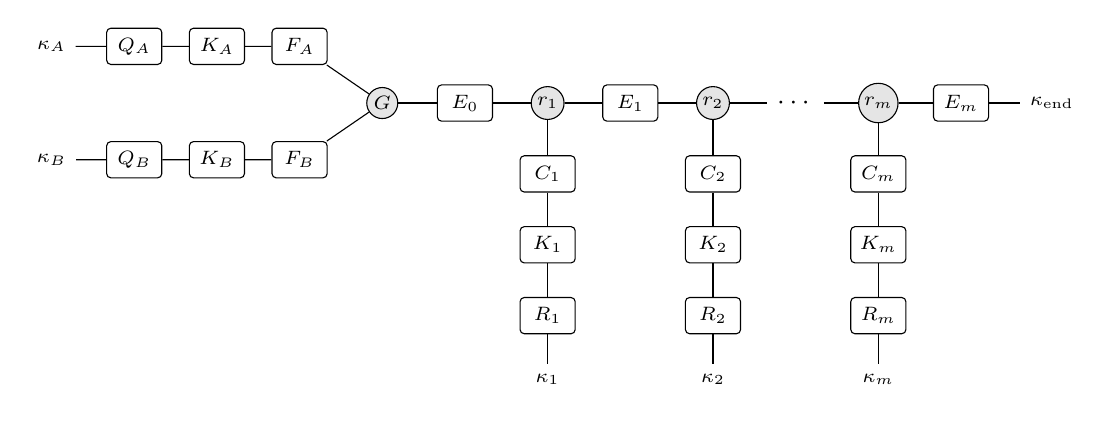
\begin{tikzpicture}[x=1.05cm,y=0.9cm,
  cell/.style={draw,rounded corners=1.5pt,minimum width=7mm,minimum height=4.6mm,font=\scriptsize,inner sep=1pt},
  jn/.style={circle,draw,fill=black!10,inner sep=1.2pt,font=\scriptsize},
  port/.style={font=\scriptsize}]
\node[jn] (G) at (0,0) {$G$};
\node[cell] (E0) at (1,0) {$E_0$};
\node[jn] (r1) at (2,0) {$r_1$};
\node[cell] (E1) at (3,0) {$E_1$};
\node[jn] (r2) at (4,0) {$r_2$};
\node (dots) at (5,0) {$\cdots$};
\node[jn] (rm) at (6,0) {$r_m$};
\node[cell] (Em) at (7,0) {$E_m$};
\node[port] (ke) at (8.1,0) {$\kend$};
\foreach \r/\x/\i in {r1/2/1,r2/4/2,rm/6/m}{
  \node[cell] (C\i) at (\x,-1) {$C_{\i}$};
  \node[cell] (K\i) at (\x,-2) {$K_{\i}$};
  \node[cell] (R\i) at (\x,-3) {$R_{\i}$};
  \node[port] (k\i) at (\x,-3.9) {$\kappa_{\i}$};
  \draw (\r)--(C\i)--(K\i)--(R\i)--(k\i);
}
\node[cell] (FA) at (-1,0.8) {$F_A$}; \node[cell] (KA) at (-2,0.8) {$K_A$};
\node[cell] (QA) at (-3,0.8) {$Q_A$}; \node[port] (kA) at (-4,0.8) {$\kappa_A$};
\node[cell] (FB) at (-1,-0.8) {$F_B$}; \node[cell] (KB) at (-2,-0.8) {$K_B$};
\node[cell] (QB) at (-3,-0.8) {$Q_B$}; \node[port] (kB) at (-4,-0.8) {$\kappa_B$};
\draw (G)--(E0)--(r1)--(E1)--(r2)--(dots)--(rm)--(Em)--(ke);
\draw (G)--(FA)--(KA)--(QA)--(kA);
\draw (G)--(FB)--(KB)--(QB)--(kB);
\end{tikzpicture}
\caption{The processor at the cell level. Each box is a two-vertex cell, each circle a junction.
Control slots are not drawn: two per cell endpoint and one per junction.}
\label{fig:processor}
\end{figure}

\begin{lemma}[Topology]\label{lem:proctopology}
$P(m)$ is a tree. Every cell endpoint and every junction has degree exactly four, and every control
slot, far clocks included, is a leaf.
\end{lemma}

\begin{proof}
At the cell level the network is a path ($G$, the bus, $\kend$) with pendant paths (the register
arms, the two temporary arms, and the far clocks). This is a tree. Each cell is an edge, each cell
adjacency is realised by exactly one edge, and the control slots are leaves. Replacing nodes of a
tree by subtrees joined through single edges gives a tree. An endpoint has its partner, one data
port (a junction, an endpoint of an adjacent cell, or a far clock) and two control slots. A
junction has three arms and one control.
\end{proof}

\begin{definition}[Phase assignment]\label{def:procphases}
Cells $E_i,C_i,R_i,F_X,Q_X$ have phase $0$; buffers $K_i,K_X$ have phase $1$; every junction control
has phase $1$; every far clock has phase $0$.
\end{definition}

This is the two-colouring of the cell-level tree, with junction controls placed on the colour
opposite to their arms. The arms of every junction have phase $0$ and its control has phase $1$.
Adjacent cells in the chains $C_i\,$--$\,K_i\,$--$\,R_i$ and $F_X\,$--$\,K_X\,$--$\,Q_X$ have opposite
phases. These are exactly the local conventions of \cref{tab:timing}, with $e=0$ for junction arms
and for the cells $A,B,C,R$ of a read, and $e\oplus1=1$ for buffers and junction controls.

\subsection{Normal configurations}

\begin{definition}[Normal configuration]\label{def:normal}
For $c\in\{0,1\}$ and $\rho:[1,m]\to\{0,1\}$, the configuration $\NORMAL(c,\rho)$ is:
\begin{itemize}
\item every bus cell $E_i=cc$, and $x_G=x_{r_i}=c$ for all $i$;
\item $C_i=K_i=bb$ and $R_i=\rho(i)\rho(i)$ for all $i$;
\item $F_A=K_A=Q_A=F_B=K_B=Q_B=bb$; the temporaries are \emph{free}.
\end{itemize}
The \emph{rest schedule of background $c$} puts every cell in \HOLD, every junction control at $c$,
and every far clock at $b$.
\end{definition}

\begin{lemma}[Stability]\label{lem:normalstable}
$\NORMAL(c,\rho)$ is a fixed point of the forced evolution under the rest schedule of background $c$.
\end{lemma}

\begin{proof}
All cells are uniform and in \HOLD\ (\cref{lem:frame}\ref{frame:hold}). The arms of $r_i$ are
$E_{i-1}=c$, $E_i=c$ and $C_i=b$, so one of them is $b$. The arms of $G$ are $E_0=c$, $F_A=b$ and
$F_B=b$, so two of them are $b$. Apply \cref{lem:frame}\ref{frame:junction}.
\end{proof}

The initial configuration of the processor is $\NORMAL(0,\rho_0)$, where $\rho_0(i)=\iota_0(i)$ for
input registers and $\rho_0(k)=0$ for instruction registers.

\subsection{One instruction}\label{sec:instruction}

Fix an instruction register $k$. Let $c=c_k$ be its background, $b=1-c$, $x=\rho(i)$,
$y=\rho(j)$, $d=x\circ_k y$, and $\rho'=\rho[k\mapsto d]$. The \emph{instruction schedule}
$\Sigma_k$ consists of the twelve phases of \cref{tab:instruction}, executed in order. Each phase
starts at the first time, not earlier than the end of the previous phase, whose parity equals the
phase's reference parity. The resulting idle step, when present, is called an \emph{alignment
wait}: it uses the rest schedule.

\begin{table}[ht]
\centering\small
\begin{tabular}{r>{\raggedright\arraybackslash}p{8.4cm}cc}\toprule
& phase (primitives, in order; $\parallel$ = simultaneous) & duration & ref.\ parity\\\midrule
1 & \prim{PREPARE}: $\prim{SET}(C_k\mathbin{:=}c)$; then $\prim{SET}(K_k\mathbin{:=}c)\parallel\prim{SET}(R_k\mathbin{:=}b)$ & $6$ & $c$\\
2 & $\prim{FETCH}(i,F_A)$ (\cref{lem:fetch}) & $12i+18$ & $c$\\
3 & \prim{STORE}: $\prim{SET}(K_A\mathbin{:=}b)$; $\prim{MOVE}_b(F_A\to K_A)$; $\prim{MOVE}_b(K_A\to Q_A)$ & $9$ & $c$\\
4 & $\prim{FETCH}(j,F_B)$ & $12j+18$ & $c$\\
5 & \prim{RECOVER}: $\prim{COPY}$ $Q_A\to K_A$ via $\FAV c$; $\prim{SET}(F_A\mathbin{:=}c)$; $\prim{MOVE}_c(K_A\to F_A)$ & $9$ & $1\oplus c$\\
6 & $\prim{GATE}_c(G;F_A,F_B\to E_0)$ & $5$ & $1\oplus c$\\
7 & \prim{CLEAN}: $\prim{SET}(Q_A\mathbin{:=}b)\parallel\prim{SET}(Q_B\mathbin{:=}b)$; then $\prim{SET}(K_A\mathbin{:=}b)\parallel\prim{SET}(K_B\mathbin{:=}b)$ & $6$ & $1\oplus c$\\
8 & \prim{LEFT}: transport $E_0\to E_{k-1}$ through $r_1,\dots,r_{k-1}$ (\cref{lem:chain}) & $6(k-1)$ & $c$\\
9 & \prim{PILOT}: $\prim{COPY}$ $\kend\to E_m$ via $\FAV b$ & $3$ & $1\oplus c$\\
10 & \prim{RIGHT}: transport $E_m\to E_k$ through $r_m,\dots,r_{k+1}$ & $6(m-k)$ & $c$\\
11 & \prim{COMMIT}: $\prim{ROUTE}(r_k;E_{k-1}\to C_k;E_k)$; $\prim{SET}(K_k\mathbin{:=}b)$; $\prim{MOVE}_b(C_k\to K_k)$; $\prim{MOVE}_b(K_k\to R_k)\parallel\prim{SET}(E_k\mathbin{:=}c)$ & $15$ & $c$\\
12 & \prim{FRONTS}: $\prim{SET}(F_A\mathbin{:=}b)\parallel\prim{SET}(F_B\mathbin{:=}b)$ & $3$ & $1\oplus c$\\\bottomrule
\end{tabular}
\caption{The instruction schedule $\Sigma_k$, for background $c=c_k$.}
\label{tab:instruction}
\end{table}

\begin{lemma}[Admissibility and alignment of $\Sigma_k$]\label{lem:sigmatiming}
With the phase assignment of \cref{def:procphases}, every block and control event of every phase of
\cref{tab:instruction} is admissible when the phase starts at its reference parity. If $\Sigma_k$
starts at a time $S\equiv c$, alignment waits occur exactly before phases $4$, $5$, $6$, $7$, $8$
and $9$, one transition each. The schedule ends at $S+D_k$ with
\[
D_k=12(i+j)+6m+92,
\]
which is even, so it ends at parity $c$.
\end{lemma}

\begin{proof}
We use \eqref{eq:startparity}, writing each event as (phase, $\zeta$, offset).
\begin{itemize}
\item Phase 1: $C_k$ $(0,0,0)$; $K_k$ $(1,0,3)$; $R_k$ $(0,1,3)$. All give $c$.
\item Phases 2 and 4: by \cref{lem:fetch} below.
\item Phase 3: $K_A$ $(1,1,0)$; $\prim{MOVE}_b(F_A\to K_A)$ $(0,1,3)$; $\prim{MOVE}_b(K_A\to Q_A)$
  $(1,1,6)$. All give $c$.
\item Phase 5: $K_A$ in $\FAV c$ $(1,0,0)$; $F_A$ $(0,0,3)$; $\prim{MOVE}_c(K_A\to F_A)$ $(1,0,6)$. All
  give $1\oplus c$.
\item Phase 6: \cref{tab:timing} with $e=0$ gives $1\oplus c$.
\item Phase 7: $Q$'s $(0,1,0)$; $K$'s $(1,1,3)$. Both give $1\oplus c$.
\item Phases 8 and 10: routes with $e=0$, at even offsets, give $c$.
\item Phase 9: $E_m$ $(0,1,0)$ gives $1\oplus c$.
\item Phase 11: route $(e=0)$ at offset $0$ gives $c$; $K_k$ $(1,1,6)$; $\prim{MOVE}_b(C_k\to K_k)$
  $(0,1,9)$; $\prim{MOVE}_b(K_k\to R_k)$ $(1,1,12)$; $E_k$ $(0,0,12)$. All give $c$.
\item Phase 12: $(0,1,0)$ gives $1\oplus c$.
\end{itemize}
Durations are $6$, even, $9$, even, $9$, $5$, $6$, even, $3$, even, $15$, $3$. Starting at parity
$c$, the end parities are $c,c,1{\oplus}c,c,c,c,1{\oplus}c,c,c,c,1{\oplus}c,c$. Comparing each end
parity with the next phase's reference parity gives one wait before phases $4,5,6,7,8,9$ and none
elsewhere. Summing,
$6+(12i+18)+9+1+(12j+18)+1+9+1+5+1+6+1+6(k-1)+1+3+6(m-k)+15+3=12(i+j)+6m+92$.
\end{proof}

\paragraph{Milestones.} \Cref{tab:milestones} lists the configuration at the end of each phase as a
difference from $\NORMAL(c,\rho)$. At every milestone all cells are uniform and in \HOLD, all
junctions are in state $c$, and all controls are at rest. In the proofs, ``$M_r$ plus $X=uu$'' means
the milestone $M_r$ with the cell $X$ replaced.

\begin{table}[ht]
\centering\small
\begin{tabular}{cl}\toprule
milestone & differences from $\NORMAL(c,\rho)$\\\midrule
$M_0$ & none\\
$M_1$ & $C_k=K_k=cc$, $R_k=bb$\\
$M_2$ & $M_1$ plus $F_A=xx$, $K_A=cc$\\
$M_3$ & $M_1$ plus $Q_A=xx$\\
$M_4$ & $M_3$ plus $F_B=yy$, $K_B=cc$\\
$M_5$ & $M_1$ plus $F_A=xx$, $K_A=cc$, $Q_A=xx$, $F_B=yy$, $K_B=cc$\\
$M_6$ & $M_1$ plus $F_A=F_B=cc$, $K_A=K_B=cc$, $Q_A=xx$, $E_0=dd$\\
$M_7$ & $M_1$ plus $F_A=F_B=cc$, $E_0=dd$\\
$M_8$ & $M_1$ plus $F_A=F_B=cc$, $E_{k-1}=dd$\\
$M_9$ & $M_8$ plus $E_m=bb$\\
$M_{10}$ & $M_8$ plus $E_k=bb$\\
$M_{11}$ & $\NORMAL(c,\rho')$ plus $F_A=F_B=cc$\\
$M_{12}$ & $\NORMAL(c,\rho')$\\\bottomrule
\end{tabular}
\caption{Milestones of $\Sigma_k$: $M_r$ is the configuration at the end of phase $r$.}
\label{tab:milestones}
\end{table}

\begin{lemma}[Alignment waits]\label{lem:waits}
Every milestone $M_r$, $0\le r\le 12$, is a fixed point of the forced evolution under the rest
schedule of background $c$. Hence the alignment waits do not change the configuration.
\end{lemma}

\begin{proof}
All cells are uniform and in \HOLD. By \cref{lem:frame} it suffices that every junction has at
most two arms in state $b$ (arms read as their adjacent endpoints).
\begin{itemize}
\item $G$, arms $(E_0,F_A,F_B)$: $(c,b,b)$ in $M_0,M_1,M_3,M_{12}$; $(c,x,b)$ in $M_2$; $(c,b,y)$
  in $M_4$; $(c,x,y)$ in $M_5$; $(d,c,c)$ in $M_6,M_7$; $(c,c,c)$ in $M_8$--$M_{11}$.
\item $r_k$: in $M_1$--$M_{10}$ its arm $C_k$ is $c$, so at most its two bus arms are $b$. In $M_0$,
  $M_{11}$ and $M_{12}$, its bus arms are $c$.
\item $r_\ell$, $\ell\ne k$: its arm $C_\ell$ is $b$, and in every milestone at most one of
  $E_{\ell-1},E_\ell$ differs from $c$. The only milestone with two non-background bus cells is
  $M_{10}$, where they are $E_{k-1}$ and $E_k$, both arms of $r_k$; and $M_9$ with $k<m$, where
  they are $E_{k-1}$ and $E_m$, which are not arms of a common junction because $k-1<m-1$.\qedhere
\end{itemize}
\end{proof}

\begin{lemma}[\prim{PREPARE}: $M_0\to M_1$]\label{lem:prepare}
Starting from $M_0$, phase~1 produces $M_1$.
\end{lemma}

\begin{proof}
During $[s,s+3)$, $C_k$ is in $\FAV c$ and its port $x_{r_k}$ is $c$ at control time $s$. The
junction $r_k$ stays $c$, since its arms are $E_{k-1}=E_k=c$ and $C_k$. By \cref{lem:forcing},
$C_k=cc$ at $s+2$ and $s+3$. During $[s+3,s+6)$, $K_k$ is in $\FAV c$ with port $\ep{C_k}{K_k}=c$ at
control time $s+3$, and $R_k$ is in $\FAV b$ with port $\kappa_k=b$. By \cref{lem:forcing}, at $s+6$
we have $K_k=cc$ and $R_k=bb$. No other cell changes.
\end{proof}

Only a fresh destination is overwritten this way: $R_k$ has not been read before instruction $k$,
and it is never read before it is written. Inputs and earlier results are never prepared.

\begin{lemma}[\prim{FETCH}]\label{lem:fetch}
Let $1\le i\le m$, let $F\in\{F_A,F_B\}$ with buffer $K_F$ and temporary $Q_F$, and let $F'$ be the
other front. Assume that at time $s$, with $s\equiv c$, all cells are uniform and in \HOLD, all
controls are at rest, and:
\begin{enumerate}[label=(\alph*)]
\item every bus cell is $cc$ and every junction is in state $c$;
\item $C_\ell=K_\ell=bb$ for all $\ell\le i$, and $R_i=xx$;
\item $F=K_F=Q_F=bb$ and $F'=bb$. The cells $K_{F'}$ and $Q_{F'}$ are arbitrary uniform cells; they
  may hold a protected value.
\end{enumerate}
Apply the schedule
\begin{center}\small
\begin{tabular}{ll}\toprule
control times & operation\\\midrule
$[s,s+6)$ & $\prim{ROUTE}(G;F\to E_0;F')$ (emit a pilot $b$)\\
$s+6$ & wait\\
$[s+7,s+10)$ & $\prim{SET}(K_F\mathbin{:=}c)$ from $F=c$\\
$[s+10,s+4+6i)$ & transport $E_0\to E_{i-1}$ through $r_1,\dots,r_{i-1}$\\
$[s+4+6i,s+18+6i)$ & $\prim{READ}(r_i;E_{i-1};C_i,K_i,R_i)$\\
$[s+18+6i,s+12+12i)$ & transport $E_{i-1}\to E_0$ through $r_{i-1},\dots,r_1$\\
$[s+12+12i,s+18+12i)$ & $\prim{ROUTE}(G;E_0\to F;F')$\\\bottomrule
\end{tabular}
\end{center}
Then at time $s+12i+18$ the configuration equals the initial one, except that $F=xx$ and
$K_F=cc$. All blocks and control events are admissible, with reference parity $c$.
\end{lemma}

\begin{proof}
Admissibility: the routes and the read have reference parity $c$ (\cref{tab:timing}, $e=0$) and
start at even offsets $0$, $10+6\ell$, $4+6i$, $18+6i+6\ell$ and $12+12i$. The block of
$\prim{SET}(K_F\mathbin{:=}c)$ is $(1,0,7)$, which also gives $c$.

\emph{Emit.} The route at $G$ has source $F=bb$, destination $E_0=cc$ and bias $F'=bb$, with
$x_G=c$. The far port of $E_0$ is $r_1$. Its arms are $E_0$, $E_1=c$ and $C_1=b$, so it stays $c$ by
the frame lemma. \Cref{lem:route} gives $F=cc$, $E_0=bb$ (the pilot) and $x_G=c$ at $s+6$.

\emph{Wait.} The configuration at $s+6$ is stable: $G$ has arms $(E_0,F,F')=(b,c,b)$, and $r_1$ has
arms $(b,c,b)$.

\emph{Buffer.} $K_F$ is in $\FAV c$ during $[s+7,s+10)$, and its port $\ep F{K_F}$ is $c$, so
\cref{lem:forcing} gives $K_F=cc$. $Q_F=bb$ is untouched.

\emph{Outward transport.} Apply \cref{lem:chain} with $X_0=E_0$ (carrying $b$), junctions
$r_1,\dots,r_{i-1}$, cells $E_1,\dots,E_{i-1}$ and biases $C_1,\dots,C_{i-1}=bb$. The final far port is
$r_i$, whose arms are $E_{i-1}$, $E_i=c$ and $C_i=b$, so it stays $c$. The vertex beyond $X_0$ is $G$,
whose arms are $E_0$, $F=c$ and $F'=b$, so it stays $c$. For $i=1$ this step is empty and the pilot
stays in $E_0$.

\emph{Read.} At time $s+4+6i$, the cells $A=E_{i-1}=bb$ (pilot), $B=E_i=cc$, $C=C_i=bb$, $K=K_i=bb$
and $R=R_i=xx$ satisfy the hypotheses of \cref{lem:read} at $g=r_i$. The far port of $A$ is $r_{i-1}$,
or $G$ if $i=1$, and it stays $c$ throughout the read. The arms of $r_{i-1}$ are $E_{i-2}=c$,
$C_{i-1}=b$ and $E_{i-1}$. The arms of $G$ are $E_0$, $F=c$ and $F'=b$. The far ports of $B$ and $R$
are irrelevant. All other junctions have unchanged arms. The read returns $E_{i-1}=xx$, $r_i=c$,
$C_i=K_i=bb$, $R_i=xx$ and $E_i=cc$.

\emph{Return transport.} Apply \cref{lem:chain} with $X_0=E_{i-1}$, with junctions
$r_{i-1},\dots,r_1$, cells $E_{i-2},\dots,E_0$ and biases $C_{i-1},\dots,C_1=bb$. The final far port is $G$, which stays
$c$ by the frame lemma, because its arms are $E_0$, $F=c$ and $F'=b$. The vertex beyond $X_0$ is
$r_i$, whose arms are $E_{i-1}$, $E_i=c$ and $C_i=b$.

\emph{Deliver.} The route at $G$ has source $E_0=xx$, destination $F=cc$ and bias $F'=bb$. The
destination's far port is $\ep{K_F}{F}=c$. The source's far port $r_1$ is arbitrary for the route;
its arms are $E_0$, $E_1=c$ and $C_1=b$, so it stays $c$. The result is $F=xx$ and $E_0=cc$.
\end{proof}

All register arms that were visited return to their normal state. The cases $i=1$ (empty transports)
and $F=F_B$ with $Q_A$ holding a value (condition (c)) are covered.

\begin{lemma}[\prim{STORE}: $M_2\to M_3$]\label{lem:store}
Starting from $M_2$, phase 3 produces $M_3$.
\end{lemma}

\begin{proof}
$\prim{SET}(K_A\mathbin{:=}b)$: its port $\ep{Q_A}{K_A}=b$ forces $K_A=bb$ (\cref{lem:forcing}), while
$F_A=xx$ is in \HOLD. Then $\prim{MOVE}_b(F_A\to K_A)$: the destination is $K_A=bb$ and its far port
is $\ep{Q_A}{K_A}=b$; the source's far port $G$ is arbitrary. \Cref{lem:move} gives $F_A=bb$ and
$K_A=xx$. Then $\prim{MOVE}_b(K_A\to Q_A)$: the destination is $Q_A=bb$ with far port $\kappa_A=b$,
giving $K_A=bb$ and $Q_A=xx$. Throughout, $G$ has $x_G=h_G=c$ and arm $E_0=c$, so it keeps $c$. The
known bit $b$ is left in front of the stored operand.
\end{proof}

At $M_3$ the front $F_A$ is $b$ and $Q_A$ holds $x$. The second fetch then runs with
$F=F_B$ and $F'=F_A=bb$, and condition (c) of \cref{lem:fetch} holds. In particular, there is no
attempt to restore $F_A$ while a pilot is in $E_0$.

\begin{lemma}[\prim{RECOVER}: $M_4\to M_5$]\label{lem:recover}
Starting from $M_4$, phase 5 produces $M_5$.
\end{lemma}

\begin{proof}
\emph{Copy.} $K_A=bb$ is in $\FAV c$. Its port on the $Q_A$ side is constantly $x$, because $Q_A$ is
in \HOLD, and its port on the $F_A$ side is constantly $b$, because $F_A=bb$ is in \HOLD. The dual form
of \cref{lem:copy} gives $K_A=xx$, and $Q_A$ is unchanged.
\emph{Clear the front.} $F_A$ is in $\FAV c$ with port $x_G=c$, so $F_A=cc$ (\cref{lem:forcing}).
\emph{Move back.} $\prim{MOVE}_c(K_A\to F_A)$: the destination is $F_A=cc$ and its far port is $x_G$;
the source's far port $Q_A$ is arbitrary. This gives $K_A=cc$ and $F_A=xx$.
During the whole phase, $x_G$, $h_G$ and the arm $E_0$ are all $c$, so $x_G=c$ is an invariant, not
an assumption about the port.
\end{proof}

\begin{lemma}[Gate step: $M_5\to M_6$]\label{lem:gatestep}
Starting from $M_5$, phase 6 produces $M_6$, with $E_0=dd$ and $d=x\circ_k y$.
\end{lemma}

\begin{proof}
Apply \cref{lem:gate} at $G$ with $A=F_A=xx$, $B=F_B=yy$ and $C=E_0=cc$. The far port of $E_0$ is
$r_1$, whose arms are $E_0$, $E_1=c$ and $C_1=b$; $C_1=b$ because $k\ge2$. So $r_1$ stays $c$. The
operands' far ports $K_A$, $K_B$ are arbitrary. The result has $E_0=dd$ and $F_A=F_B=cc$. The result
is already on the bus, so no third temporary is needed.
\end{proof}

\begin{lemma}[\prim{CLEAN}: $M_6\to M_7$]\label{lem:clean}
Starting from $M_6$, phase 7 produces $M_7$.
\end{lemma}

\begin{proof}
$Q_A$ and $Q_B$ are forced to $bb$ through their far clocks, which are $b$; then $K_A$ and $K_B$ are
forced to $bb$ through $\ep{Q_X}{K_X}=b$ (\cref{lem:forcing}). These cells are not arms of $G$, and $G$
keeps $c$ because $F_A=F_B=c$.
\end{proof}

\begin{remark}[Why the fronts stay at $c$]\label{rem:fronts}
While $E_0$ holds $d$, the fronts must remain $c$. If $d=b$ and both fronts were restored to $b$, then
$G$ would have three arms in state $b$ and would flip. Restoring the buffers and temporaries early is
harmless, because they are not arms of $G$. The fronts are restored in phase 12, after $E_0=c$.
\end{remark}

\begin{lemma}[Writing routes: $M_7\to M_{10}$]\label{lem:writeroutes}
Starting from $M_7$, phases 8, 9 and 10 produce $M_8$, $M_9$ and $M_{10}$ in turn. Throughout, the
packets stay on opposite sides of $r_k$ and never cross it.
\end{lemma}

\begin{proof}
\emph{Left.} Apply \cref{lem:chain} with $X_0=E_0$ (carrying $d$), junctions $r_1,\dots,r_{k-1}$ and
biases $C_1,\dots,C_{k-1}=bb$. Every traversed arm has bias $b$, including the arms read in phases 2
and 4: since $i,j<k$, the prepared arm $C_k=c$ is not traversed. The final far port is $r_k$, whose
arms are $E_{k-1}$, $E_k=c$ and $C_k=c$, so it stays $c$ even if $d=b$. The vertex beyond $X_0$ is
$G$, whose arms are $F_A=F_B=c$, so it stays $c$.

\emph{Pilot.} $E_m=cc$ is in $\FAV b$, with port $\kend=b$ constant and other port $x_{r_m}$. The
junction $r_m$ stays $c$. If $k=m$, its arms are $E_{m-1}=d$, $C_m=c$ and $E_m$. If $k<m$, its arms
are $E_{m-1}=c$, $C_m=b$ and $E_m$. By \cref{lem:copy}, $E_m=bb$.

\emph{Right.} If $k<m$, apply \cref{lem:chain} with $X_0=E_m$ (carrying $b$), junctions
$r_m,\dots,r_{k+1}$, cells $E_{m-1},\dots,E_k=cc$ and biases $C_m,\dots,C_{k+1}=bb$. The final far port
is $r_k$, whose arms are $E_{k-1}=d$, $C_k=c$ and $E_k$, so it stays $c$. Beyond $X_0$ is the
external port $\kend$. If $k=m$ the phase is empty and $M_9=M_{10}$.

While both packets wait next to $r_k$, the arm $C_k=c$ keeps $r_k$ at $c$ even when $d=b$. Leaving
$C_k=b$ would not have this property; this is why the destination is prepared before the fetches.
\end{proof}

\begin{lemma}[\prim{COMMIT}: $M_{10}\to M_{11}$]\label{lem:commit}
Starting from $M_{10}$ at time $s$, phase 11 produces $M_{11}$ at $s+15$: $E_{k-1}=E_k=cc$,
$C_k=K_k=bb$, $R_k=dd$ and $x_{r_k}=c$.
\end{lemma}

\begin{proof}
\emph{$[s,s+6)$: route.} \Cref{lem:route} at $r_k$, with source $E_{k-1}=dd$, destination $C_k=cc$,
bias $E_k=bb$ and $x_{r_k}=c$. The destination's far port is $\ep{K_k}{C_k}=c$. The source's far port
is $r_{k-1}$ (which exists because $k\ge 2$); its arms are $E_{k-2}=c$, $C_{k-1}=b$ and
$E_{k-1}$, so it stays $c$. Result: $C_k=dd$, $E_{k-1}=cc$.

\emph{$[s+6,s+9)$: buffer.} $K_k$ is in $\FAV b$, with port $\ep{R_k}{K_k}=b$, so $K_k=bb$. The
junction $r_k$ has arms $E_{k-1}=c$, $E_k=b$ and $C_k=d$, so it stays $c$.

\emph{$[s+9,s+12)$: first move.} $\prim{MOVE}_b(C_k\to K_k)$: the destination is $K_k=bb$ and its far
port is $\ep{R_k}{K_k}=b$; the source's far port $r_k$ is arbitrary. Result: $C_k=bb$ and $K_k=dd$.
The isolator $C_k$ is restored while the datum advances. The junction $r_k$ keeps $c$, because
$x_{r_k}$, $h_k$ and $E_{k-1}$ are $c$.

\emph{$[s+12,s+15)$: second move and pilot erasure.} $\prim{MOVE}_b(K_k\to R_k)$: the destination is
$R_k=bb$ and its far port is $\kappa_k=b$. Result: $K_k=bb$ and $R_k=dd$. Simultaneously $E_k$ is in
$\FAV c$ with port $x_{r_k}=c$, so $E_k=cc$; its other port, $r_{k+1}$ or $\kend$ when $k=m$, may be
arbitrary. During erasure, $x_{r_k}$, $h_k$ and $E_{k-1}$ are all $c$, so even $C_k=E_k=b$ cannot flip
$r_k$. If $k<m$, the junction $r_{k+1}$ has arms $E_k$, $E_{k+1}=c$ and $C_{k+1}=b$, so it stays $c$.
\end{proof}

Restoration happens \emph{during} transport: the first move restores $C_k$ while advancing the
datum, and the second restores $K_k$ while writing $R_k$. It does not happen after a uniform
channel has joined two equal stored values.

\begin{lemma}[\prim{FRONTS}: $M_{11}\to M_{12}$]\label{lem:fronts}
Starting from $M_{11}$, phase 12 produces $M_{12}$, which is $\NORMAL(c,\rho')$.
\end{lemma}

\begin{proof}
$F_A$ and $F_B$ are forced to $bb$ through $\ep{K_X}{F_X}=b$. The junction $G$ keeps $c$, because
$x_G$, $h_G$ and $E_0$ are $c$.
\end{proof}

\begin{proposition}[Instruction step]\label{prop:instruction}
Let $k$ be an instruction register and $c=c_k$. If the processor is in $\NORMAL(c,\rho)$ at a time
$S\equiv c$ and $\Sigma_k$ is applied from $S$, then it is in $\NORMAL(c,\rho[k\mapsto
\rho(i)\circ_k\rho(j)])$ at time $S+D_k$, where $D_k=12(i+j)+6m+92$. All blocks and control events
of $\Sigma_k$ are admissible. The schedule $\Sigma_k$ depends only on $k$, $i$, $j$ and $\circ_k$,
not on $\rho$.
\end{proposition}

\begin{proof}
Chain \cref{lem:prepare,lem:fetch,lem:store,lem:recover,lem:gatestep,lem:clean,lem:writeroutes,lem:commit,lem:fronts},
with the waits justified by \cref{lem:waits} and the timing by \cref{lem:sigmatiming}. The fetch
lemma applies in phase 2 at $M_1$: $C_\ell=K_\ell=bb$ for $\ell\le i$ because $k>i$. It applies in
phase 4 at $M_3$ because $k>j$, $F_B=K_B=Q_B=bb$ and $F_A=bb$. When $i=j$, the first read restored
$C_i$, $K_i$ and $R_i$ before the second read. No step consults the bits $x$, $y$ or $d$.
\end{proof}

\subsection{Changing the background}\label{sec:normalize}

\begin{lemma}[\prim{NORMALIZE}]\label{lem:normalize}
Suppose the processor is in $\NORMAL(c,\rho)$ at a time $s_0\equiv c$. Put $t_0=s_0+6$,
$t_j=t_0+4(m-j)$ for $1\le j\le m$, and $s=t_0+4m$. Apply:
\begin{center}\small
\begin{tabular}{ll}\toprule
control times & modes and controls\\\midrule
$[s_0,s_0+3)$ & $\prim{SET}(F_A\mathbin{:=}c)$\\
$[s_0+3,t_0)$ & $\prim{COPY}$ $\kend\to E_m$ via $\FAV b$\\
from $t_0$ on & every far clock changes from $b$ to $c$\\
$[t_j,t_j+3)$ & $C_j$ in $\FAV c$; $h_j$ changes from $c$ to $b$ at $t_j$ and stays $b$\\
$[t_j+1,t_j+4)$ & $K_j$ in $\FAV c$, $E_{j-1}$ in $\FAV b$\\
$[s,s+3)$ & $F_A,F_B,Q_A,Q_B$ in $\FAV c$; $h_G$ changes to $b$ at $s$ and stays $b$\\
$[s+1,s+4)$ & $K_A,K_B$ in $\FAV c$\\\bottomrule
\end{tabular}
\end{center}
Then at time $s+4=s_0+4m+10$ the processor is in $\NORMAL(b,\rho)$, and the controls are at the rest
values of background $b$. All blocks and control events are admissible. Every register $R_i$ stays
in \HOLD\ throughout.
\end{lemma}

\begin{proof}
\emph{Admissibility}, by \eqref{eq:startparity} with background $c$. The events are: $F_A$
$(0,0,0)$; $E_m$ $(0,1,3)$; the far clocks $(0,0,6)$; at offset $a_j=6+4(m-j)$, $C_j$ $(0,0,a_j)$
and $h_j$ $(1,1,a_j)$; $K_j$ $(1,0,a_j+1)$ and $E_{j-1}$ $(0,1,a_j+1)$; at offset $a=6+4m$, $F,Q$
$(0,0,a)$ and $h_G$ $(1,1,a)$; and $K$'s $(1,0,a+1)$. All give $c$.

\emph{Preparing the left end.} $\prim{SET}(F_A\mathbin{:=}c)$ through $x_G=c$; $G$ keeps $c$ because
its arm $E_0$ and $h_G$ are $c$. This step prevents the future arrival of $E_0=b$ from meeting two
fronts already equal to $b$, which would flip $G$ prematurely.

\emph{Seeding.} $E_m=cc$ in $\FAV b$ with port $\kend=b$ and other port $x_{r_m}=c$. The junction
$r_m$ stays $c$, since its arms are $E_{m-1}=c$, $C_m=b$ and $E_m$. \Cref{lem:copy} gives $E_m=bb$ at
$t_0$. At $t_0$ the far clocks switch to $c$. At that moment every cell whose port is a far clock,
namely $R_i$, $Q_A$, $Q_B$ and $E_m$, is uniform and in \HOLD, so the switch changes no state; in
particular the seed $E_m=bb$ is kept.

\emph{The wave.} For $j=m,m-1,\dots,1$ we prove the invariant $W_j$ at time $t_j$:
$E_m,\dots,E_j=bb$ and $E_{j-1},\dots,E_0=cc$; $x_{r_\ell}=h_\ell=b$ and $C_\ell=K_\ell=cc$ for
$\ell>j$; $x_{r_\ell}=c$ and $C_\ell=K_\ell=bb$ for $\ell\le j$, where $h_\ell$ is still at rest
$c$ before control time $t_\ell$; $F_A=cc$,
$F_B=K_A=K_B=Q_A=Q_B=bb$ and $x_G=h_G=c$; the registers are unchanged; and every cell is in \HOLD.
$W_m$ holds at $t_0=t_m$. Assume $W_j$. For $c=0$, the states of $r_j$ and of the endpoints of
$E_{j-1}$, $C_j$, $K_j$, with $y=\rho(j)$, are:
\begin{center}\small
\begin{tabular}{cccccccc}\toprule
time & $x_{r_j}$ & $\ep{E_{j-1}}{r_j}$ & $\ep{E_{j-1}}{\mathrm{far}}$ & $\ep{C_j}{r_j}$ & $\ep{C_j}{K_j}$ & $\ep{K_j}{C_j}$ & $\ep{K_j}{R_j}$\\\midrule
$t_j$   & $0$ & $0$ & $0$ & $1$ & $1$ & $1$ & $1$\\
$t_j+1$ & $1$ & $0$ & $0$ & $0$ & $1$ & $1$ & $1$\\
$t_j+2$ & $1$ & $1$ & $0$ & $0$ & $0$ & $1$ & $y$\\
$t_j+3$ & $1$ & $1$ & $1$ & $0$ & $0$ & $0$ & $y$\\
$t_j+4$ & $1$ & $1$ & $1$ & $0$ & $0$ & $0$ & $0$\\\bottomrule
\end{tabular}
\end{center}
At control time $t_j$, $r_j$ reads the incoming $E_j=b$, the old $C_j=b$ and $h_j=b$, so it becomes
$b$. Simultaneously $\ep{C_j}{r_j}=\AND(1,1,x_{r_j}{=}0)=0$ reads the old $r_j=c$. Afterwards the
self-vote, $E_j$ and $h_j$ keep $r_j=b$. $C_j$ is cleared from its junction side and $K_j$ from its
$C_j$ side, one step later. The endpoint $\ep{K_j}{R_j}$ temporarily reads the register bit $y$, and is
cleared at $t_j+3$ through its partner. $E_{j-1}$ in $\OR_3$ captures $r_j=1$ and becomes uniform. At
control time $t_j+3$, $C_j$ is in \HOLD\ and uniform $00$, so it stays $00$ although its port $r_j$ is
$1$. $R_j$ is in \HOLD\ and uniform throughout.

Frame: the next junction $r_{j-1}$, if $j\ge 2$, has arms $E_{j-2}=c$, $C_{j-1}=b$ and $E_{j-1}$, so
it keeps $c$ and cannot flip early. If $j=1$ the next junction is $G$, whose arms are $E_0$, $F_A=c$
and $F_B=b$: again at most two are $b$, and this is why $F_A$ was set to $c$. Junctions $r_\ell$ with
$\ell>j$ have $x_{r_\ell}=h_\ell=b$ and arm $E_\ell=b$, so they keep $b$. Hence $W_{j-1}$ holds at
$t_j+4=t_{j-1}$.

\emph{The left end.} At $s=t_0+4m$ the invariant $W_0$ holds: all bus cells and all $r_\ell$ are $b$,
$E_0=bb$, and $G$ waits at $c$ with arms $(E_0,F_A,F_B)=(b,c,b)$. For $c=0$:
\begin{center}\small
\begin{tabular}{cccccc}\toprule
time & $x_G$ & $F_B$ & $Q_X$ & $K_A$ & $K_B$\\\midrule
$s$   & $0$ & $(1,1)$ & $(1,1)$ & $(1,1)$ & $(1,1)$\\
$s+1$ & $1$ & $(0,1)$ & $(1,0)$ & $(1,1)$ & $(1,1)$\\
$s+2$ & $1$ & $(0,0)$ & $(0,0)$ & $(0,1)$ & $(1,1)$\\
$s+3$ & $1$ & $(0,0)$ & $(0,0)$ & $(0,0)$ & $(0,0)$\\
$s+4$ & $1$ & $(0,0)$ & $(0,0)$ & $(0,0)$ & $(0,0)$\\\bottomrule
\end{tabular}
\end{center}
Here $F_B$ is listed as ($G$-side, $K_B$-side), $Q_X$ as ($K_X$-side, $\kappa_X$-side), and $K_X$ as
($F_X$-side, $Q_X$-side); $F_A=00$ throughout.
At control time $s$, $G$ reads $E_0=b$, the old $F_B=b$ and $h_G=b$, so it becomes $b$. At the same
time $\ep{F_B}G$ is cleared by the old $x_G=c$. Afterwards the self-vote, $E_0$ and $h_G$ keep $G$ at
$b$. Each temporary is cleared through its new far clock $c$, and each buffer is cleared from its two
ends during $[s+1,s+4)$.

At $s+4$: every bus cell is $bb$; all junctions and all controls are $b$; $C_\ell=K_\ell=cc$;
$F,K,Q=cc$; the far clocks are $c$; and the registers are unchanged. This is $\NORMAL(b,\rho)$. The
duration is $3+3+4m+4=4m+10$, with no internal waits.
\end{proof}

\subsection{The program and its invariant}\label{sec:program}

\begin{definition}[Program schedule]\label{def:programschedule}
The program schedule $\Sigma(\mathcal P)$ starts at time $0$ in the configuration
$\NORMAL(0,\rho_0)$, with current background $0$. For each instruction register $k$ in increasing order:
\begin{enumerate}[label=(\roman*)]
\item if $c_k$ differs from the current background, apply \prim{NORMALIZE} (\cref{lem:normalize}),
  followed by one alignment wait, and update the current background;
\item apply $\Sigma_k$.
\end{enumerate}
After the last instruction, apply the rest schedule of background $c_m=0$ up to the horizon $\Hz$.
Let $\tau_k$ be the time at which $\Sigma_k$ ends, and $\tau=\tau_m$.
\end{definition}

\begin{corollary}[Observation time]\label{cor:tau}
Let $k_1<k_2<\dots$ be the instruction registers, and put $c_{k_0}=0$. Then
\[
\tau=\sum_{k}\Bigl(12(i_k+j_k)+6m+92+(4m+11)\cdot\one\{c_k\ne c_{k^-}\}\Bigr),
\]
where $k^-$ is the instruction preceding $k$, and $c_{k^-}=0$ for the first instruction. In
particular $\tau\le(m-1)(34m+79)\le 34m^2+79m$.
\end{corollary}

\begin{proof}
A normalisation lasts $4m+10$ and starts at parity $c$. It ends at parity $c$, while the next
$\Sigma_k$ must start at the new reference parity $b$; this costs exactly one wait. Each $\Sigma_k$
starts and ends at parity $c_k$ (\cref{lem:sigmatiming}), and normalisation starts at parity $c$, so
no other waits occur between instructions. For the bound, use $i_k,j_k\le m-1$, at most $m-1$
instructions, and $24(m-1)+6m+92+4m+11=34m+79$.
\end{proof}

\begin{theorem}[Forced-control simulation]\label{thm:forced}
Let $\Hz\ge\tau+3$. In the forced evolution of the processor under $\Sigma(\mathcal P)$ on $[0,\Hz]$:
\begin{enumerate}[label=(\alph*)]
\item\label{forced:inv} at time $\tau_k$ the configuration is $\NORMAL(c_k,\rho_{k})$, where
  $\rho_{k}$ is the register content after executing the instructions up to $k$, with the unexecuted
  instruction registers equal to $0$;
\item\label{forced:out} $R_m=\val(\mathcal P)\val(\mathcal P)$ at every time in $[\tau,\Hz+1]$;
\item\label{forced:phase} every control word, of every cell slot, junction control and far clock, is
  phased for its assigned phase on $[0,\Hz]$;
\item\label{forced:oblivious} $\Sigma(\mathcal P)$ depends only on the instruction types and the
  operand indices of $\mathcal P$, not on $\iota_0$.
\end{enumerate}
\end{theorem}

\begin{proof}
\ref{forced:inv} By induction over the instructions. Initially we are in $\NORMAL(0,\rho_0)$ at time
$0$, of parity $0=c$. If a normalisation is needed, \cref{lem:normalize} moves $\NORMAL(c,\rho)$ to
$\NORMAL(c_k,\rho)$, and the wait is harmless by \cref{lem:normalstable}. Then
\cref{prop:instruction} adds the value of $R_k$. The invariant fixes all register contents: the
previous values are preserved, because they are untouched except by reads, which preserve them.

\ref{forced:out} At $\tau$ the configuration is $\NORMAL(0,\rho_m)$ with
$\rho_m(m)=\rho_m(o)\wedge\rho_m(o)=\val(\mathcal P)$. It is a fixed point of the rest schedule
(\cref{lem:normalstable}).

\ref{forced:phase} Each phase consists of primitives whose blocks and control events are admissible
(\cref{lem:sigmatiming,lem:fetch,lem:normalize}). Phases are executed one after the other. Inside a
phase, simultaneous blocks lie on distinct cells, so the blocks on any one cell are pairwise
disjoint. By \cref{lem:concat} the slot words of every cell are phased. Junction controls change only
inside routes, gates and reads, and in normalisations; far clocks change only in normalisations. All
these events are admissible, so \cref{lem:bitphase} applies. At time $0$ no constraint applies.
After $\tau$ the words are constant.

\ref{forced:oblivious} \Cref{tab:instruction}, the normalisation rule and the waits are determined by
$m$ and by $(k,i_k,j_k,\circ_k)$ for each $k$.
\end{proof}

\begin{remark}[Boundary cases]\label{rem:boundary}
The case $i=j$ is included: the first read leaves the source intact and restores its isolators
before the second read. The case $i=1$ is covered by the fetch lemma, with empty bus traversals. The
case $k=m$ is covered by the pilot and right-transport arguments of \cref{lem:writeroutes} and by
the commit, where the other port of $E_k$ is $\kend$. Input registers may be interleaved with
instruction registers. Fan-out is implemented by repeated fetches, without additional data edges and
without expansion into a formula.
\end{remark}

% ====================================================================
\section{Reduction analysis}\label{sec:analysis}
% ====================================================================

Fix an MSLP $\mathcal P$ in normal form with $m$ registers, its program schedule
$\Sigma(\mathcal P)$, its observation time $\tau$ (\cref{cor:tau}), and the horizon $\Hz=\tau+3$.
Any polynomial $\Hz\ge\tau+3$ works equally well; the original manuscript uses
$\Hz=10000(m+1)^2$.

\begin{construction}[The output tree]\label{con:tree}
For every control slot $\sigma$ of $P(m)$ (two per cell endpoint, one per junction, one per far
clock), let $w_\sigma$ be its word under $\Sigma(\mathcal P)$ on $[0,\Hz]$ and $\beta_\sigma$ its
phase (\cref{def:procphases}). Let $\Gamma_\sigma=\Gamma\bigl(D(w_\sigma,\beta_\sigma),\beta_\sigma\bigr)$
(\cref{cor:words}), with private vertex names. The tree $T$ is obtained from $P(m)$ by identifying
each slot with the root of its generator, as in \cref{prop:substitution}. Its initial configuration
is $\NORMAL(0,\rho_0)$ on the processor vertices and the initial bits of the generators elsewhere. The
designated vertex $v^\ast$ is the endpoint $\ep{R_m}{K_m}$, and the query time is $\tau$.
\end{construction}

\subsection{Correctness}

\begin{proposition}[Correctness]\label{prop:correct}
In the majority evolution of $T$, $x_{v^\ast}(\tau)=\val(\mathcal P)$. More precisely, the
processor vertices of $T$ follow the forced evolution of \cref{thm:forced} at all times in
$[0,\Hz+1]$.
\end{proposition}

\begin{proof}
By \cref{thm:forced}\ref{forced:phase}, every $w_\sigma$ is $\beta_\sigma$-phased. By
\cref{cor:words}, $\Gamma_\sigma$ is a robust generator whose root history agrees with $w_\sigma$ on
$[0,\Hz]$. \Cref{prop:substitution}\ref{sub:same} shows that the processor vertices follow the forced
evolution up to time $\Hz+1\ge\tau$, and \cref{thm:forced}\ref{forced:out} gives the value.
\end{proof}

We now spell out the three properties of the clock trees that the proof relies on.
\begin{itemize}
\item \emph{Autonomy.} Each generator is a private subtree, joined to the processor by one edge, and
  robust. Its root history is fixed in advance, whatever the processor does, including feedback
  through the consumer (\cref{def:robust,prop:substitution}). No control schedule is an input of the
  dynamics, and no vertex is forced from outside during the evolution: $T$ with $x(0)$ is a closed,
  autonomous system.
\item \emph{Compatibility with the operations.} Every word demanded by the operations is realisable
  by a fixed-phase generator. This is \cref{thm:forced}\ref{forced:phase}, proved through the
  cell-phase and concatenation lemmas, the timing signatures, and the explicit alignment waits.
  Every constant control during \HOLD\ is also supplied by a generator over the whole horizon.
\item \emph{Constructibility.} See \cref{prop:logspace} below.
\end{itemize}

\subsection{Degree, acyclicity and size}

\begin{proposition}[Topology]\label{prop:topology}
$T$ is a tree, and every vertex of $T$ has degree $1$, $3$ or $4$.
\end{proposition}

\begin{proof}
$P(m)$ is a tree whose slots are leaves (\cref{lem:proctopology}). By
\cref{prop:substitution}\ref{sub:tree}, $T$ is a tree, the processor vertices keep degree four, and
every generator vertex keeps its degree in $\{1,3,4\}$, consumer edge included (\cref{cor:words}).
No two generators share a vertex, and no root is identified with another root.
\end{proof}

\begin{proposition}[Size]\label{prop:size}
$|V(T)|=O(m\,\Hz^{\alpha+3})=O(m^{2\alpha+7})\subseteq O(m^{13})$.
\end{proposition}

\begin{proof}
The processor has $4m+7$ cells and $m+1$ junctions. It therefore has $4(4m+7)+(m+1)+(m+3)=O(m)$
control slots: four per cell, two at each endpoint; one per junction; and $m+3$ far clocks. Each
generator has size $O((\Hz+2)^{\alpha+3})$ by \cref{cor:words}, and $\Hz=\tau+3=O(m^2)$ by
\cref{cor:tau}. Since $\alpha<3$, the exponent satisfies $2\alpha+7<13$. The bound is conservative,
not optimised, and $T$ is listed explicitly, not described succinctly.
\end{proof}

\subsection{Logspace constructibility}

\begin{proposition}[Logspace transducer]\label{prop:logspace}
The map $\mathcal P\mapsto(T,x(0),v^\ast,\tau)$ is computable in space $O(\log m)$, hence in
logarithmic space in the length of the encoding of $\mathcal P$.
\end{proposition}

\begin{proof}
We describe three subroutines, each using $O(\log m)$ bits of work space, and compose them.

\emph{(1) Schedule interpretation.} Given a slot $\sigma$ and a time $t\le\Hz$, the bit
$w_\sigma(t)$ is computed by scanning the program schedule. Keep a time counter, the current
instruction register $k$, its operands $i_k,j_k$ (reread from the input when needed), the current
background, the index of the current phase of \cref{tab:instruction} or of the normalisation, and
route or wave counters. These are $O(1)$ integers below $\Hz+m$. Each phase has a known duration,
and each alignment wait is decided by a parity comparison, so the scan advances phase by phase until
the phase containing $t$ is found. The value of $\sigma$ at $t$ is then read off the phase
description: a mode of the cell, a control value, or the rest value of the current background. Only
the current bit of the queried slot is stored. Nothing depends on the values in the registers: the
scan never evaluates the program (\cref{rem:twospaces}). The same scan, run to the end, computes
$\tau$, which is written in binary.

\emph{(2) Processor emission.} The cells, junctions, endpoints, slots and edges of $P(m)$ are
indexed by $O(\log m)$-bit names, and the initial bits $\NORMAL(0,\rho_0)$ are read from $\iota_0$.
Phases are given by \cref{def:procphases}.

\emph{(3) Generator emission.} For each slot $\sigma$, run the procedure of \cref{lem:genlogspace} with
$\beta=\beta_\sigma$ and the membership oracle $t\in D(w_\sigma,\beta_\sigma)$, which is
$w_\sigma(t)\ne\beta_\sigma\oplus(t\bmod2)$ and is answered by subroutine (1). It uses
$O(\log(\Hz+2))=O(\log m)$ bits. Generator vertex names are prefixed by the name of $\sigma$, and the
root is emitted with the name of the slot, which realises the identification of
\cref{prop:substitution}.

Composition: subroutine (3) calls (1) as an oracle, recomputing answers on demand. The composition of
logspace computations is computable in logspace~\cite{Jon75,LL76}. Because $\Hz$ is polynomial in
$m$, all counters stay within $O(\log m)$ bits.
\end{proof}

\begin{proof}[Proof of \cref{thm:simulation}, prediction part]
Items~\ref{sim:tree} and~\ref{sim:size} are \cref{prop:topology,prop:size}; \ref{sim:time} is
\cref{cor:tau}; \ref{sim:correct} is \cref{prop:correct}. Logspace computability is
\cref{prop:logspace}. The extension to arbitrary MSLPs composes with \cref{lem:normalform}. The
eventual-activation part is proved in \cref{sec:ever}.
\end{proof}

% ====================================================================
\section{Completeness results}\label{sec:completeness}
% ====================================================================

\subsection{Membership in P, including binary-encoded times}\label{sec:membership}

The following is the classical bounded-transient argument for symmetric majority networks
\cite{GO80,PS83,GFP85}. We include the proof because we need the explicit transient bound for
binary-encoded times, in the exact model of \cref{def:majority}. It applies to every explicit
instance, not only to the constructed trees.

\begin{proposition}[Membership]\label{prop:membership}
Let $T$ be a finite simple undirected graph with $n$ vertices, and let $W=2|E|+n$. For every initial
configuration, $x(t+2)=x(t)$ for all $t\ge W$. Consequently, $\Pred$ and $\Ever$ are in $\Ptime$, even
when $\tau$ is a large binary integer.
\end{proposition}

\begin{proof}
Use spins $s_v=2x_v-1\in\{-1,1\}$. Put $w_{vu}=w_{uv}=1$ for each edge, $w_{vv}=1$ when $\deg(v)$ is
even (including degree zero), and all other weights $0$. No physical self-loop is added; the diagonal
is used only for the analysis. Every row sum $\sum_u w_{vu}$ is odd, and
\begin{equation}\label{eq:sign}
s_v(t+1)=\operatorname{sign}\Bigl(\sum_u w_{vu}s_u(t)\Bigr),
\end{equation}
because at even degree the diagonal term breaks exactly the ties, and at odd degree there are no
ties. Define
\[
\Phi(t)=\sum_{v,u}w_{vu}\,s_v(t+1)\,s_u(t),\qquad |\Phi(t)|\le\sum_{v,u}w_{vu}=W.
\]
By the symmetry of $w$,
\begin{equation}\label{eq:energy}
\Phi(t+1)-\Phi(t)=\sum_v\bigl(s_v(t+2)-s_v(t)\bigr)\sum_u w_{vu}s_u(t+1).
\end{equation}
The inner sum is an odd integer with sign $s_v(t+2)$ by \eqref{eq:sign}. So each term is $0$ if
$s_v(t+2)=s_v(t)$ and at least $2$ otherwise. Let $t^\ast$ be the first $t$ with $x(t+2)=x(t)$. By
determinism, $x(t+2)=x(t)$ for all $t\ge t^\ast$, and for $t<t^\ast$, $\Phi$ increases by at least $2$
at each step. Since $\Phi$ takes values in $[-W,W]$, we get $2t^\ast\le 2W$.

Algorithm for $\Pred$: simulate up to time $W+1$, which is at most $3n$ for a tree. If $\tau\le W+1$, answer $x_{v^\ast}(\tau)$;
otherwise answer $x_{v^\ast}(W+((\tau-W)\bmod 2))$, using only the parity of $\tau$. Algorithm for
$\Ever$: the states after $W$ repeat with period dividing two, so $z$ is ever $1$ if and only if
$x_z(t)=1$ for some $1\le t\le W+1$. Both run in time polynomial in the explicit input length.
\end{proof}

\subsection{Prediction}

\begin{proof}[Proof of \cref{thmB}]
Membership: \cref{prop:membership}. Hardness: given an instance of $\OMCVP$, which is
$\Ptime$-complete by \cref{thm:mcvp}, \cref{thm:simulation} produces in logspace an instance
$(T,x(0),v^\ast,\tau)$ of $\Pred$ with degrees in $\{1,3,4\}$, polynomial $\tau$, and
$x_{v^\ast}(\tau)=1$ if and only if the circuit outputs $1$. Composition of logspace reductions
\cite{Jon75,LL76} completes the proof.
\end{proof}

\subsection{Eventual activation}\label{sec:ever}

The clock theorem implements the processor controls only up to a finite horizon. After $\Hz$ the
generators alternate, and the processor may behave arbitrarily (\cref{rem:afterH}). Prediction at the
single time $\tau$ is unaffected, but eventual activation is not: a false instance must never
activate the designated vertex, even after $\Hz$. We need a reader that rejects in the false case
whatever happens outside its window.

\begin{lemma}[Finite-window reader]\label{lem:reader}
Let $q$ be a vertex with an arbitrary history, except that $x_q(T_0)=x_q(T_0+1)=d$. Attach a new
vertex $z$ adjacent to $q$, to a private leaf $\ell$, and to the roots of two private copies of
$P_{T_0,T_0+2}$ (\cref{lem:pulses}). Initialise $z=\ell=0$. Then $z$ has degree four, $\ell$ has
degree one, the pulses use degrees $1$ and $3$, and the edge $qz$ counts towards the degree of $q$.
Moreover:
\begin{enumerate}[label=(\alph*)]
\item $x_z(t)=0$ for all $t\le T_0$, whatever the history of $q$;
\item $x_z(t)=1$ for some $t$ if and only if $d=1$, in which case $x_z(T_0+1)=1$.
\end{enumerate}
\end{lemma}

\begin{proof}
The pulses are robust and their consumer is $z$, so both are $1$ exactly at times $T_0$ and $T_0+1$,
and $0$ at all other times, \emph{including all times after $T_0+1$}: their tail is exactly zero for
every $t\ge T_0+2$. Before $T_0$, if $z=\ell=0$ then only $q$ can vote one at $z$, so $z$ stays $0$,
and the leaf copies $z$. Hence $z=\ell=0$ up to time $T_0$. At control time $T_0$,
$x_z(T_0+1)=\MAJ_5(0,d,0,1,1)=d$ and $x_\ell(T_0+1)=0$. At $T_0+1$,
$x_z(T_0+2)=\MAJ_5(d,d,0,1,1)=d$ and $x_\ell(T_0+2)=d$. From control time $T_0+2$ on, both pulses
are $0$. If $d=0$, the invariant $z=\ell=0$ is restored at $T_0+2$ and persists for every later
history of $q$, since only $q$ can vote one. If $d=1$, the witness $x_z(T_0+1)=1$ has occurred;
retaining $1$ forever is not needed.
\end{proof}

The reader does not require the input to start at zero, nor that it was never $1$ earlier. Nor does
it require the phase-defect clocks to keep \HOLD\ forever.

\begin{construction}[The activation tree]\label{con:ever}
Let $\mathcal P$ be in normal form; its last instruction is $R_m\leftarrow R_o\wedge R_o$, of
background $0$. Modify \cref{con:tree} as follows.
\begin{enumerate}[label=(\arabic*)]
\item \emph{Reader at the far port.} Remove the far clock $\kappa_m$, and attach the reader vertex $z$
  of \cref{lem:reader} to $q=\ep{R_m}{\kappa_m}$, in the same data port. This adds no edge at the
  register endpoint, which still has degree four.
\item \emph{Final instruction.} In $\Sigma_m$, omit $\prim{SET}(R_m\mathbin{:=}b)$ from
  \prim{PREPARE}, so that $R_m$ stays $00$ and only $C_m=K_m=00$ are prepared. Replace phases 11
  and 12 by the \emph{final write}:
  \begin{align*}
  &\prim{ROUTE}(r_m;E_{m-1}\to C_m;E_m) &&\text{during }[s,s+6),\\
  &\prim{MOVE}_0(C_m\to K_m) &&\text{during }[s+6,s+9),\\
  &\prim{MOVE}_0(K_m\to R_m) &&\text{during }[s+9,s+12),
  \end{align*}
  starting at the end $s$ of phase 10, which is empty since $k=m$. Let $\tau_E=s+12$, and keep the
  rest schedule of background $0$ afterwards.
\item \emph{Window.} Use $T_0=\tau_E$ in the reader, and the horizon $\Hz=\tau_E+3$ for all
  generators.
\end{enumerate}
The designated vertex is $z$, with $x_z(0)=0$.
\end{construction}

\begin{lemma}[Final write]\label{lem:finalwrite}
In the activation tree, the processor vertices follow the forced evolution of the modified schedule
up to time $\Hz+1$. At times $\tau_E$ and $\tau_E+1$, $R_m=dd$ with $d=\val(\mathcal P)$. All blocks
and control events of the modified schedule are admissible.
\end{lemma}

\begin{proof}
\emph{Before the final instruction.} The port of $\ep{R_m}{\kappa_m}$ now carries $x_z$ instead of a
far clock. By \cref{lem:reader}(a), $x_z(t)=0$ for $t\le\tau_E$, for every history of $R_m$. The cell
$R_m$ is in \HOLD\ and uniform $00$ from time $0$ until the last move. It is never read, because every
operand index is smaller than $m$. It is not prepared, and normalisation leaves registers in \HOLD.
So the content of its far port is never used before the final write, and
\cref{lem:prepare,lem:fetch,lem:normalize,prop:instruction} hold verbatim for all instructions
$k<m$. Within $\Sigma_m$, phases 1 to 10 are as before, except that $R_m=00$ instead of $bb$; these
phases never involve $R_m$. No read enters the branch of $R_m$.

\emph{Final write ($c=0$, $b=1$).} At $s$ we have $E_{m-1}=dd$, $E_m=11$ (the pilot), $C_m=K_m=00$,
$R_m=00$ and $x_{r_m}=0$. The route has destination $C_m=00$, whose far port is $\ep{K_m}{C_m}=0$, and
bias $E_m=11$. Its source's far port is $r_{m-1}$, whose arms are $E_{m-2}=0$, $C_{m-1}=1$ and
$E_{m-1}$, so it stays $0$. By \cref{lem:route}, $C_m=dd$ and $E_{m-1}=00$. Then
$\prim{MOVE}_0(C_m\to K_m)$: the destination is $K_m=00$ with far port $\ep{R_m}{K_m}=0$, which gives
$C_m=00$ and $K_m=dd$. Then $\prim{MOVE}_0(K_m\to R_m)$: the destination is $R_m=00$, and its far
port is $x_z$, which is $0$ at control times $\tau_E-3,\tau_E-2,\tau_E-1\le\tau_E$. This gives
$K_m=00$ and $R_m=dd$ at $\tau_E$. During these moves $r_m$ keeps $0$, because its self-vote, $h_m$
and $E_{m-1}=0$ are $0$. Afterwards $R_m$ is in \HOLD\ and uniform, so it holds $dd$ at $\tau_E+1$,
whatever $z$ does. Since this is the final write, neither restoring $C_m,K_m$ nor returning the whole
processor to a normal configuration is needed.

\emph{Admissibility.} The route at $r_m$ has reference parity $c=0$, and phase 10 ends at parity $0$
(\cref{lem:sigmatiming}). $\prim{MOVE}_0(C_m\to K_m)$ is the event $(0,0,6)$, and
$\prim{MOVE}_0(K_m\to R_m)$ is $(1,0,9)$. Both give $0$ by \eqref{eq:startparity}. The omitted
$\prim{SET}(R_m\mathbin{:=}b)$ only removes a block. The conclusions of \cref{thm:forced}\ref{forced:phase}
and of \cref{prop:correct} therefore hold for the modified schedule, with $\Hz=\tau_E+3$.
\end{proof}

\begin{proof}[Proof of \cref{thmC} and of the activation part of \cref{thm:simulation}]
\emph{Topology and size.} The activation tree is obtained from a tree with the far clock $\kappa_m$
removed by attaching the reader through the single edge $qz$. The reader is itself a tree, with
$z$ of degree four, $\ell$ of degree one, and pulses with degrees $1$ and $3$. So it is a tree with
degrees in $\{1,3,4\}$. The two pulses have size $O((\tau_E+3)^2)$.

\emph{Correctness.} By \cref{lem:finalwrite}, $x_q(\tau_E)=x_q(\tau_E+1)=d=\val(\mathcal P)$ in the
closed tree. By \cref{lem:reader}, $z$ is ever $1$ if and only if $d=1$. If the program outputs $0$,
then $z$ stays $0$ forever, even though the phase-defect clocks alternate after $\Hz$ and may change
the processor arbitrarily.

\emph{Uniformity.} The reader and its pulses are emitted in logspace (\cref{lem:genlogspace}, or
directly from the explicit description of \cref{lem:pulses}), and the modified schedule is
interpreted as in \cref{prop:logspace}.

\emph{Completeness.} Membership is \cref{prop:membership}, and hardness follows from \cref{thm:mcvp}
as in the proof of \cref{thmB}.
\end{proof}

\subsection{Scope}

\begin{remark}\label{rem:scope}
\begin{itemize}
\item The construction proves hardness already at treewidth one.
\item It does not show that four is the smallest possible maximum degree. The classification at
  maximum degree three remains unresolved in the source notes.
\item The construction of degree five with only odd degrees is a separate, earlier result.
\item Nothing here separates $\Ptime$ from $\NC$, and no claim of bibliographic priority or
  external validation is made.
\end{itemize}
\end{remark}


\appendix
% ====================================================================
\section{Correspondence with the original manuscript}\label{app:map}
% ====================================================================

The table maps every section of the original manuscript~\cite{Src} to its place in this version.
Nothing of mathematical substance was removed. The appendix on source files and internal review status,
which is not mathematical, is summarised at the end of this appendix.

\begin{center}\small
\begin{longtable}{p{4.6cm}p{4.6cm}p{5.2cm}}\toprule
original & this version & change\\\midrule\endhead
\S1 model, Def.~1.1, Thm.~1.2 & \cref{sec:prelim}, \cref{def:problems}, \cref{thmB,thmC} & split into model and results\\
\S1 source problem (ordered MCVP) & \cref{sec:model,sec:pcomplete} & recast as MSLPs; classical references made explicit; normal-form lemma added\\
\S2.1 robust generators, constant sources & \cref{def:robust}, \cref{sec:timers} & feedback made explicit in the definition\\
Lemma 2.1 (timers) & \cref{lem:timers} & unchanged\\
Lemma 2.2 (pulses) & \cref{lem:pulses} & unchanged\\
Thm.~2.3 (phase defects) & \cref{thm:phasedefect} & unchanged\\
\S2.4 combiner & \cref{lem:combiner} & three cases merged into two\\
\S2.5 bases, size & proof of \cref{thm:phasedefect}, \cref{lem:paritytransform} & parity transformation isolated as a lemma\\
\S2.6 logspace enumeration & \cref{lem:genlogspace} & unchanged\\
\S2.7 realised words & \cref{lem:charwords}, \cref{cor:words} & unchanged\\
\S3.1 \textsf{EDGE} cell, Lemma 3.1 & \cref{lem:modes,lem:forcing,lem:copy} & forcing hypothesis weakened (\cref{rem:forcing-hyp})\\
\S3.2 move & \cref{lem:move}, \cref{rem:nopause} & unchanged\\
\S3.3 junction, routing & \cref{lem:route}, \cref{lem:frame} & frame lemma factored out; chain transport \cref{lem:chain} added\\
\S3.4 gates & \cref{lem:gate} & unchanged\\
\S3.5 phase assignment & \cref{sec:phasecalc}, \cref{def:procphases} & cell-phase, concatenation and timing lemmas\\
\S4 read (Lemma 4.1), \S4.2 & \cref{lem:read}, \cref{tab:timing} & unchanged; timing via the calculus\\
\S5.1 processor, normal form & \cref{def:processor,def:normal,lem:proctopology,lem:normalstable} & stability made a lemma\\
\S5.2 alignment waits & \cref{lem:sigmatiming,lem:waits} & waits enumerated; stability of each waiting configuration proved\\
\S5.3 prepare, commit & \cref{lem:prepare,lem:commit} & unchanged\\
\S5.4 fetch, store, recover & \cref{lem:fetch,lem:store,lem:recover} & fetch proved through \cref{lem:chain}\\
\S5.5 gate, cleanup, routes & \cref{lem:gatestep,lem:clean,lem:writeroutes}, \cref{rem:fronts} & unchanged\\
\S5.6 normalisation & \cref{lem:normalize} & wave invariant $W_j$ made explicit\\
\S5.7 program invariant & \cref{prop:instruction,thm:forced}, \cref{tab:milestones} & milestones tabulated; closed formula for $\tau$ (\cref{cor:tau})\\
\S6.1 control replacement & \cref{prop:substitution,prop:correct} & substitution principle stated and proved\\
\S6.2 size and time & \cref{prop:size}, \cref{cor:tau} & horizon $\Hz=\tau+3$, or any larger polynomial\\
\S6.3 logspace transducer & \cref{prop:logspace} & unchanged\\
\S7 membership in $\Ptime$ & \cref{prop:membership} & attributed to the classical energy method\\
\S8.1 reader (Lemma 8.1) & \cref{lem:reader} & unchanged\\
\S8.2 final write & \cref{con:ever}, \cref{lem:finalwrite} & unchanged\\
Scope paragraph & \cref{rem:scope} & unchanged\\\bottomrule
\end{longtable}
\end{center}

\paragraph{Provenance.} The original English edition assembles research notes dated 8 October
2026. Those notes record internal readings of the reduction and are attributed there to automated
research agents. No human authorship, publication status, independent external review or
proof-assistant verification is asserted there, and none is asserted here. The present version is a
reorganisation; the computational checks of \cref{app:audit} are sanity checks, not part of the
proof.

% ====================================================================
\section{Audit notes}\label{app:audit}
% ====================================================================

\paragraph{Points made explicit by the reorganisation.}
\begin{enumerate}[label=(\arabic*)]
\item \emph{Duality.} ``Complementing the contract'' is formalised at the level of modes
  (\cref{lem:duality}). Literal complementation of control bits would replace $\HOLD=(0,1)$ by
  $(1,0)$ (\cref{rem:dualcontrols}). Duality shifts the admissible start parity by one, which is the
  background term $c$ in \eqref{eq:startparity}.
\item \emph{Merging of control blocks.} The phase rule of the original requires each mode block to
  start at the right parity and to have odd length. It does not address two adjacent blocks of the
  same mode, which would merge into one block of even length and violate \eqref{eq:phase}.
  \Cref{lem:concat} proves that this cannot happen when all blocks are admissible.
\item \emph{Alignment waits.} The original permits ``a zero- or one-transition wait whenever the
  preparation is stable''. Here the waits are determined exactly (\cref{lem:sigmatiming}): six per
  instruction plus one after each normalisation. The stability of every waiting configuration is
  proved (\cref{lem:waits}), and the observation time follows in closed form (\cref{cor:tau}).
\item \emph{Feedback through consumers.} Robustness quantifies over all consumer histories, so it
  covers feedback. The substitution principle (\cref{prop:substitution}) makes the induction
  explicit.
\item \emph{Frame conditions.} Every junction outside the footprint of a primitive is checked
  through \cref{lem:frame} in the corresponding proof. For bus transports, the far ports of
  intermediate destinations are handled once and for all inside \cref{lem:chain}.
\item \emph{Space bounds.} The space of the reduction is kept separate from the complexity of
  evaluation (\cref{rem:twospaces}).
\end{enumerate}
No error affecting the validity of the original argument was found: every schedule of the original
is reproduced unchanged.

\paragraph{Computational sanity checks.} Two scripts accompany this version, in
\texttt{tools/check/}. They re-implement the constructions from the text.
\begin{itemize}
\item \texttt{processor\_sim.py} simulates the processor at vertex level, with every control slot
  forced to its scheduled word. It checks:
  \begin{itemize}
  \item every milestone $\NORMAL(c_k,\rho_k)$ and the output;
  \item condition \eqref{eq:phase} for every control word, with its assigned phase;
  \item the absence of overlapping mode assignments;
  \item the formula $D_k=12(i+j)+6m+92$;
  \item the activation variant, including arbitrary perturbations of $R_m$ after the window.
  \end{itemize}
  It runs on all programs in normal form with at most three source nodes, plus the appended final
  gate, and on random programs with up to ten registers. Deliberate mutations are detected: omitting
  $\prim{SET}(F_A\mathbin{:=}c)$ in normalisation, a pause inside a move, removing the internal
  wait of a fetch, a read that does not restore $C$, and restoring the fronts before $E_0=c$.
\item \texttt{clock\_sim.py} builds the timers, the pulses and the phase-defect generators exactly as
  described, and simulates them against adaptive and adversarial consumers. It checks the degrees,
  that each output is a tree, the timer sizes, the counting recurrence \eqref{eq:counting} at every
  skeleton node, \cref{lem:charwords}, and \cref{lem:reader}. The generators are checked for all defect
  sets with dates at most $11$, in both phases, and for random larger ones.
\end{itemize}
These checks support the written proofs but do not replace them. The complete trees, of size
$O(m^{13})$, are not simulated end to end. The link between the forced processor and the
generators is \cref{prop:substitution}, which is proved, not tested.


\begin{thebibliography}{99}\small

\bibitem[GFP85]{GFP85}
E.~Goles-Chacc, F.~Fogelman-Souli\'e, and D.~Pellegrin.
\newblock Decreasing energy functions as a tool for studying threshold networks.
\newblock \emph{Discrete Applied Mathematics}, 12(3):261--277, 1985.

\bibitem[GO80]{GO80}
E.~Goles and J.~Olivos.
\newblock Periodic behaviour of generalized threshold functions.
\newblock \emph{Discrete Mathematics}, 30(2):187--189, 1980.

\bibitem[GHR95]{GHR95}
R.~Greenlaw, H.~J. Hoover, and W.~L. Ruzzo.
\newblock \emph{Limits to Parallel Computation: {P}-Completeness Theory}.
\newblock Oxford University Press, 1995.

\bibitem[Gol77]{Gol77}
L.~M. Goldschlager.
\newblock The monotone and planar circuit value problems are log space complete for {P}.
\newblock \emph{SIGACT News}, 9(2):25--29, 1977.

\bibitem[Jon75]{Jon75}
N.~D. Jones.
\newblock Space-bounded reducibility among combinatorial problems.
\newblock \emph{Journal of Computer and System Sciences}, 11(1):68--85, 1975.

\bibitem[Lad75]{Lad75}
R.~E. Ladner.
\newblock The circuit value problem is log space complete for {P}.
\newblock \emph{SIGACT News}, 7(1):18--20, 1975.

\bibitem[LL76]{LL76}
R.~E. Ladner and N.~A. Lynch.
\newblock Relativization of questions about log space computability.
\newblock \emph{Mathematical Systems Theory}, 10:19--32, 1976.

\bibitem[PS83]{PS83}
S.~Poljak and M.~S\r{u}ra.
\newblock On periodical behaviour in societies with symmetric influences.
\newblock \emph{Combinatorica}, 3(1):119--121, 1983.

\bibitem[Src]{Src}
Source notes of the original manuscript.
\newblock \emph{P-Completeness of Synchronous Majority on Trees of Maximum Degree Four}, English
edition of 13 November 2026, compiled from research notes dated 8 October 2026. Its ordered circuit
convention refers to Section~3.1 and Proposition~3.3 of arXiv:2610.04311v1.

\end{thebibliography}

\end{document}
